\section{Evaluation results}
\label{sec:ch4-report}

The report generated by fuzzbench collecting the coverage information is placed in \texttt{report-data} directory, beside the experiment files located in \texttt{xp-data}. The reports are generated in figures and an HTML file for illustrating the results. We first analyze the code coverages, and then we examine the execution times.

\subsection{Code coverage}

Figure \ref{fig:cov-growth} shows the code coverage growth of the fuzzers, while fuzzing each benchmark. There are three trials for each fuzzer, and the illustration shows the highest code coverage, the minimum code coverage, and the median of the trials' results. AFL++ shows a significant better performance than other benchmarks. In fact, AFL++ is has the highest performance in coverage among all other benchmarks which are provided in fuzzbench project. Waffle, as expected, is seemingly performing same as AFL. This is followed by the fact that Waffle performs the same code coverage approach, but there are new different features for producing queue entries. In \ref{fig:sub:freetype-cov-growth}, the trials of Waffle show more variance in performance. Hence, AFL's trials grow close to each other. In the paper based on fuzzbench results \cite{metzman2021fuzzbench}, the \texttt{deterministic stages} of AFL's fuzzing is behind such performance. It is also noticeable that Waffle discovers significantly more regions in at least one of the trials. Testing libjpeg-turbo-07-2017 (Figure \ref{fig:sub:libjpeg-cov-growth}) and libpng-1.2.56 (Figure \ref{fig:sub:libpng-cov-growth}) show a close performance for AFL, AFLFast, and Waffle \ref{fig:sub:libjpeg-cov-growth}. Another interesting result collected from fuzzing libxml2-v2.9.2 suggests a difficulty for Waffle in exploring the code coverage, but eventually Waffle gets the pace closer to other fuzzers. In addition, AFL is the winner of the 4th experiment.

\begin{figure}
    \centering
    \begin{subfigure}[t]{\textwidth}
        \centering
        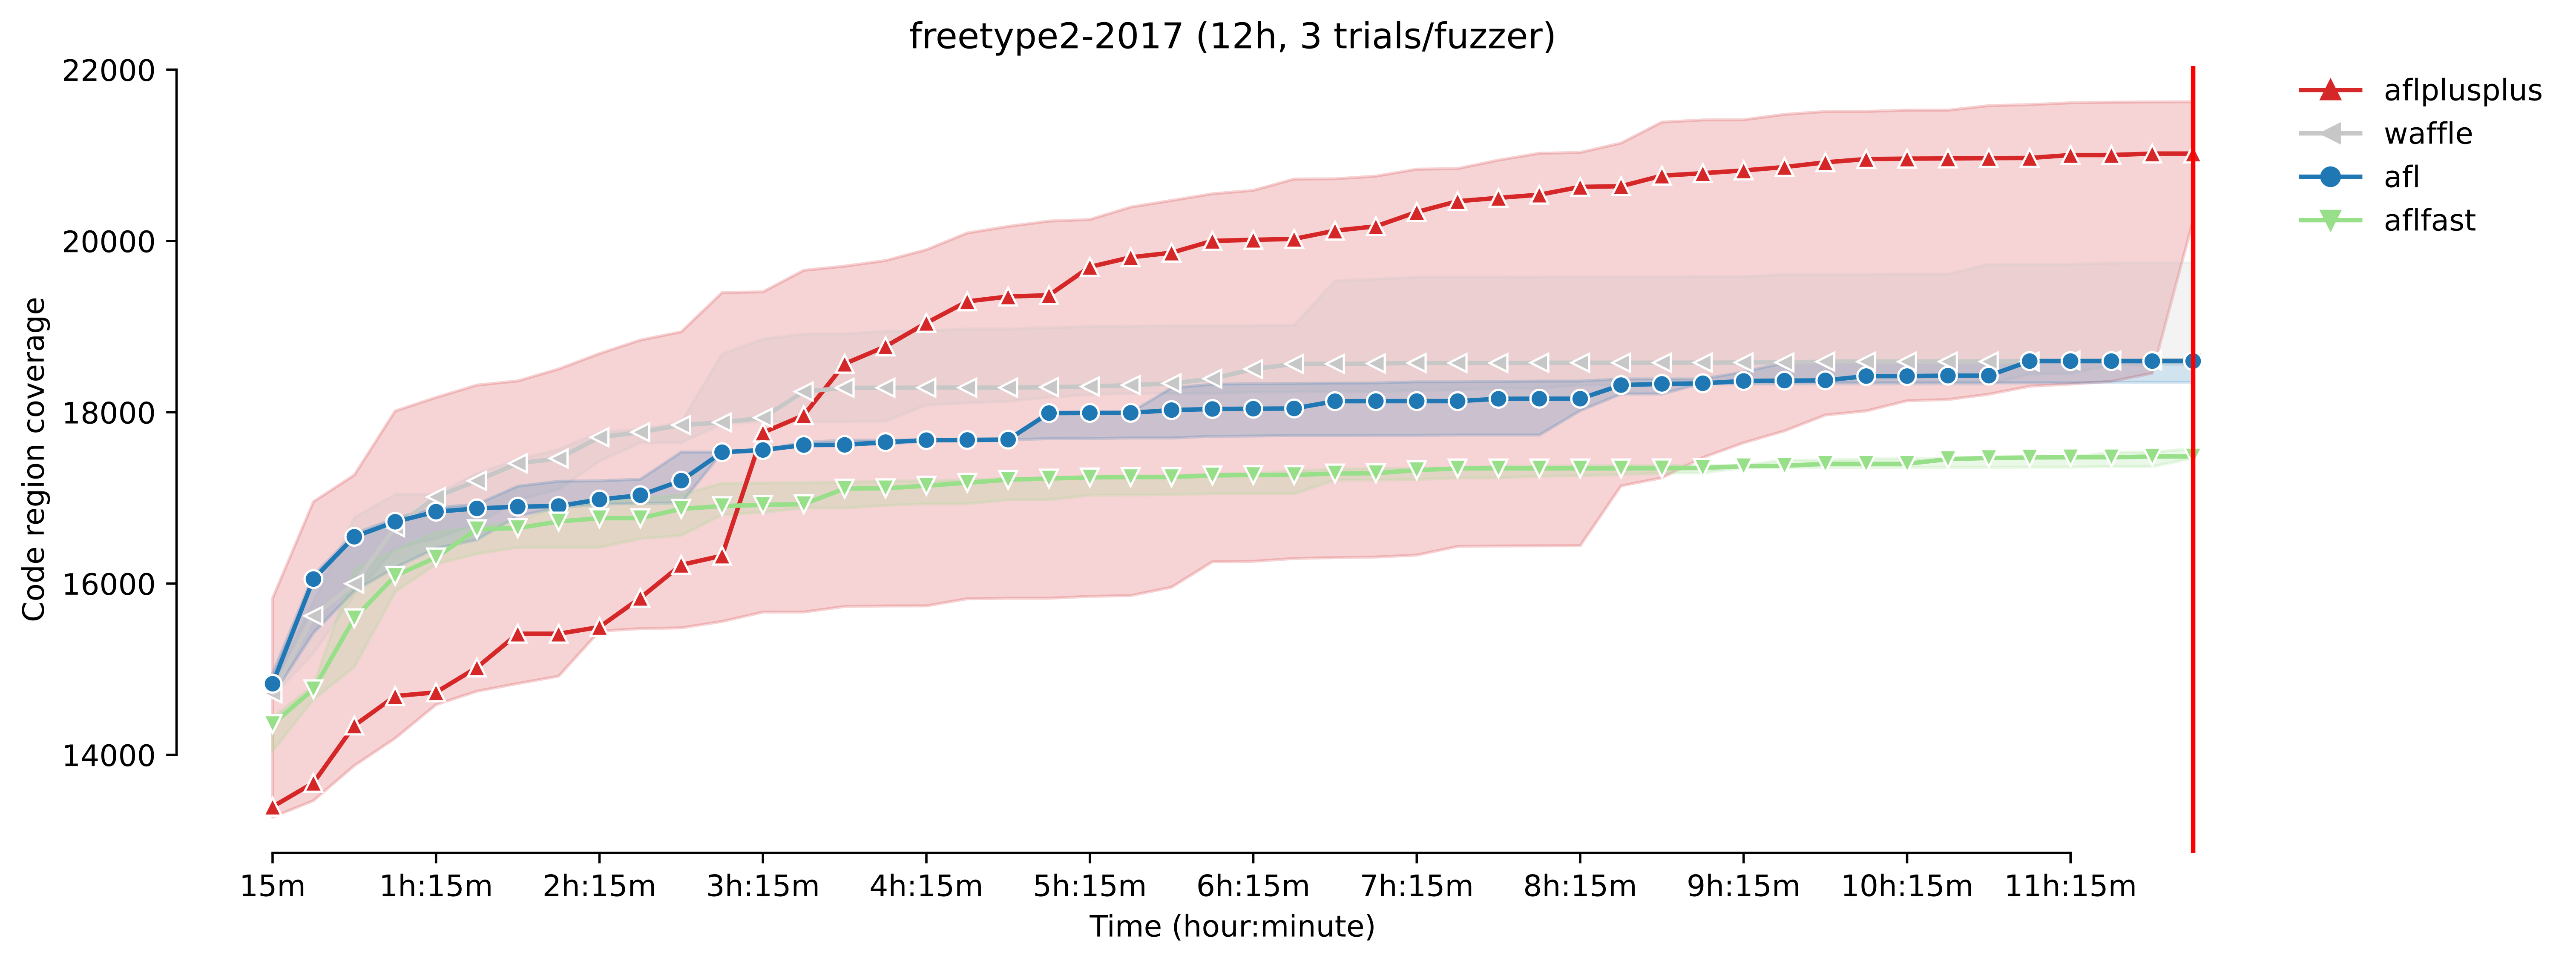
\includegraphics[width=0.85\textwidth]{Experiments/freetype2-2017_coverage_growth.png}
        \caption{freetype2-2017}
        \label{fig:sub:freetype-cov-growth}
    \end{subfigure}

    \begin{subfigure}[t]{\textwidth}
        \centering
        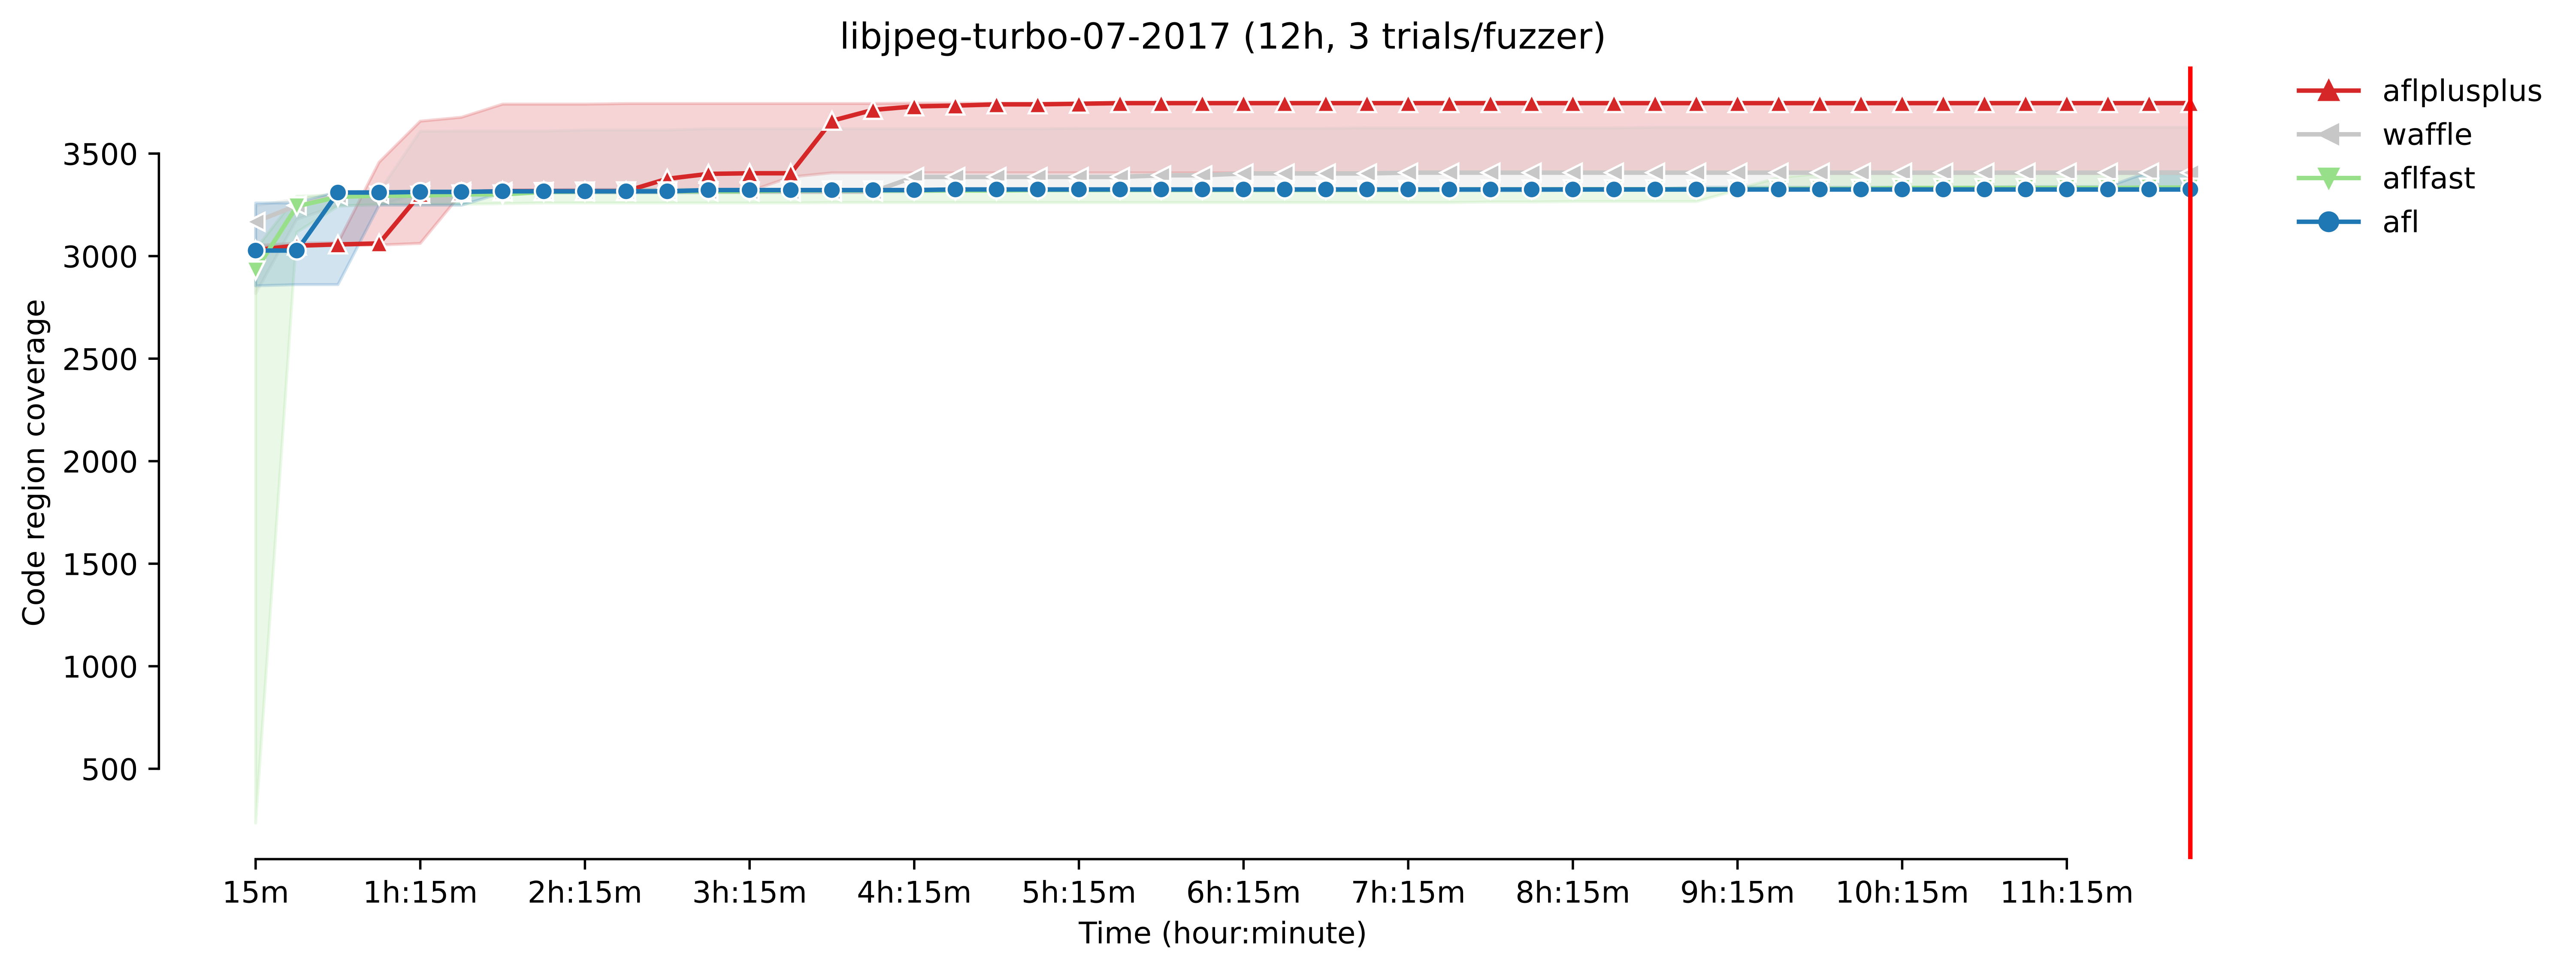
\includegraphics[width=0.85\textwidth]{Experiments/libjpeg-turbo-07-2017_coverage_growth.png}
        \caption{libjpeg-turbo-07-2017}
        \label{fig:sub:libjpeg-cov-growth}
    \end{subfigure}

    \begin{subfigure}[t]{\textwidth}
        \centering
        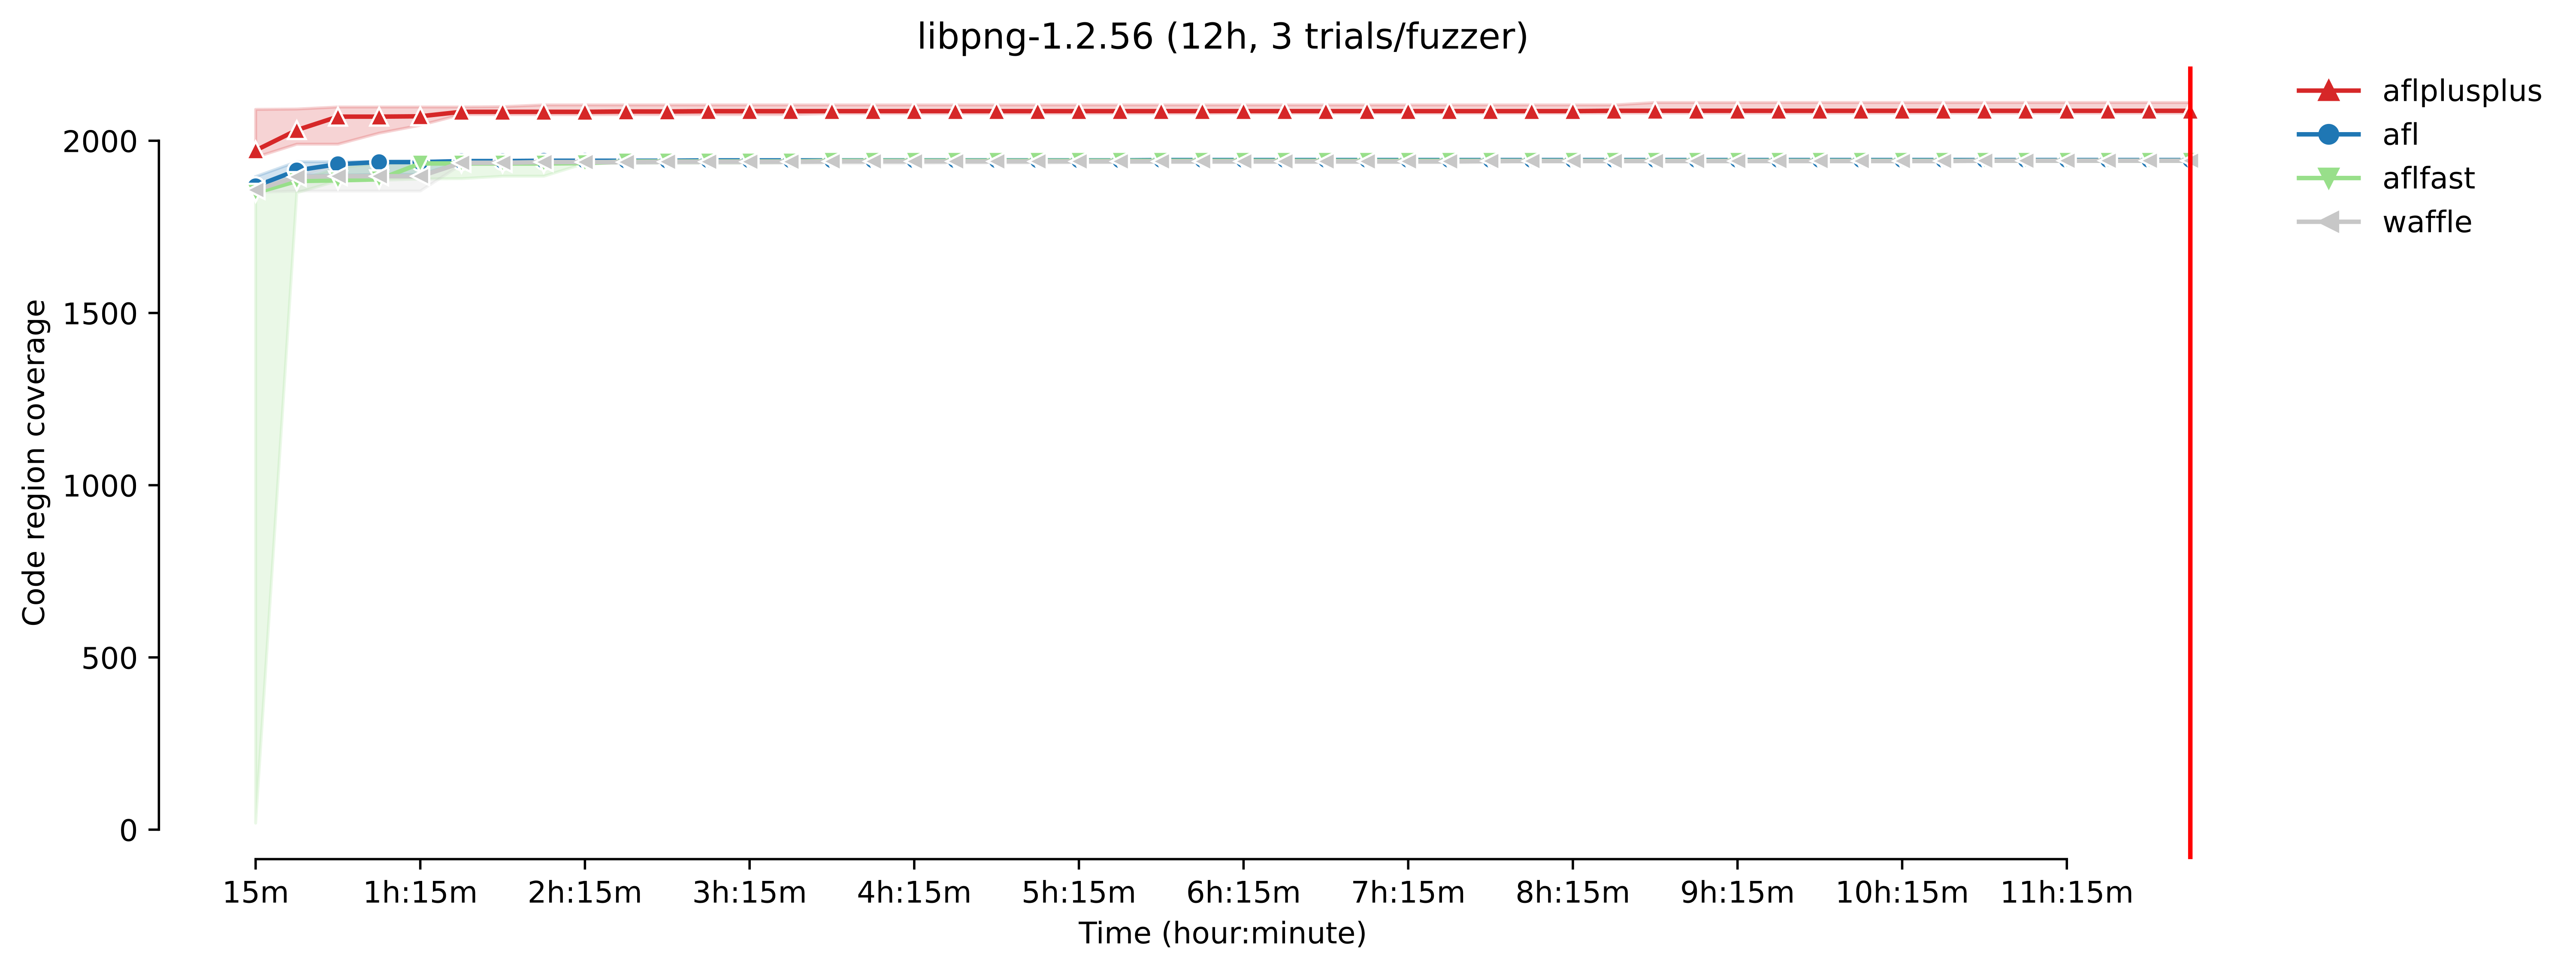
\includegraphics[width=0.85\textwidth]{Experiments/libpng-1.2.56_coverage_growth.png}
        \caption{libpng-1.2.56}
        \label{fig:sub:libpng-cov-growth}
    \end{subfigure}

    \begin{subfigure}[t]{\textwidth}
        \centering
        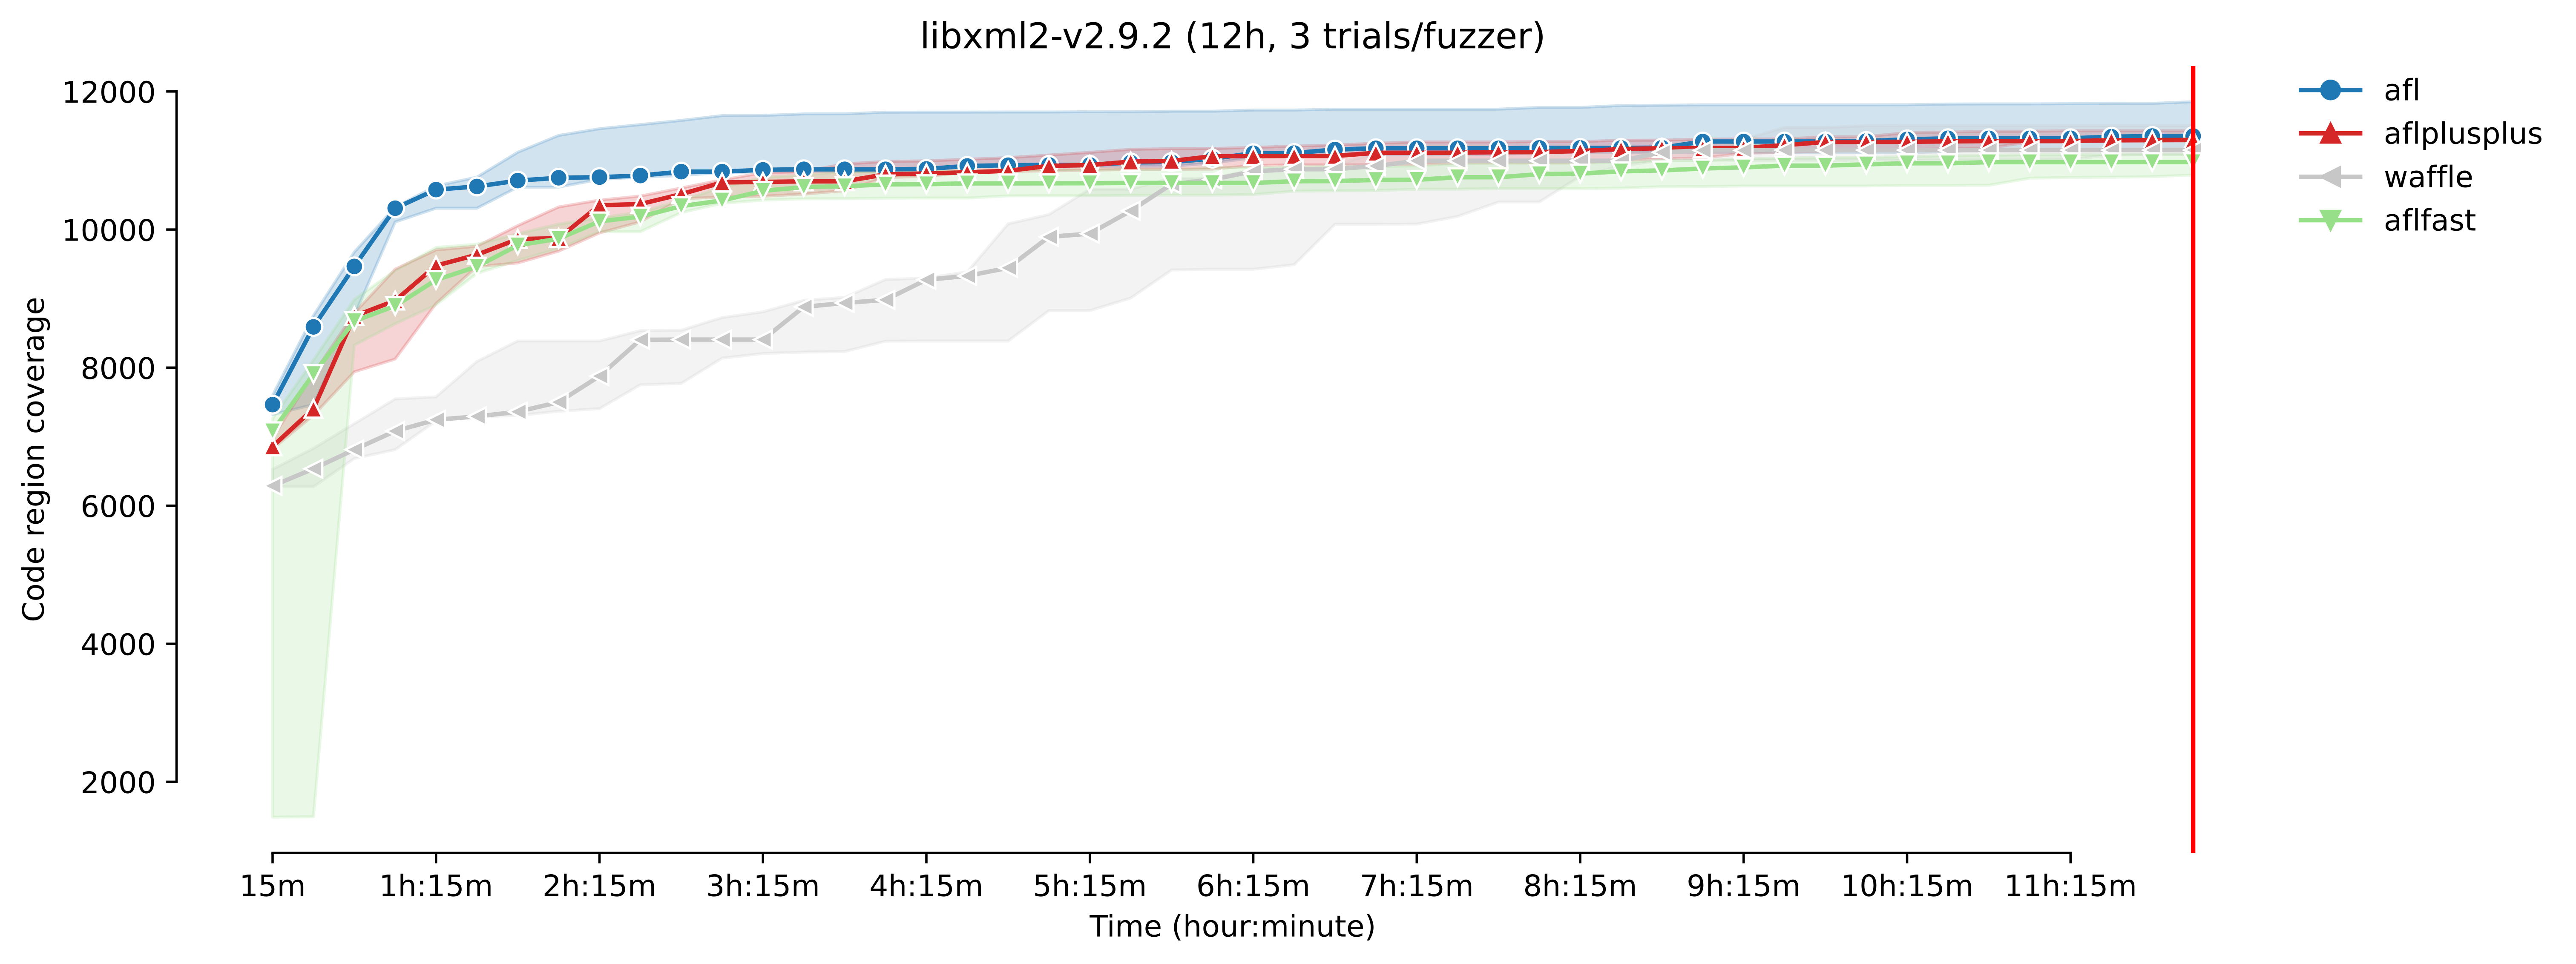
\includegraphics[width=0.85\textwidth]{Experiments/libxml2-v2.9.2_coverage_growth.png}
        \caption{libxml2-v2.9.2}
        \label{fig:sub:libxml-cov-growth}
    \end{subfigure}

    \caption{Coverage growth during the trials}
    \label{fig:cov-growth}
\end{figure}



\begin{figure}
    \centering
    \begin{subfigure}[t]{\textwidth}
        \centering
        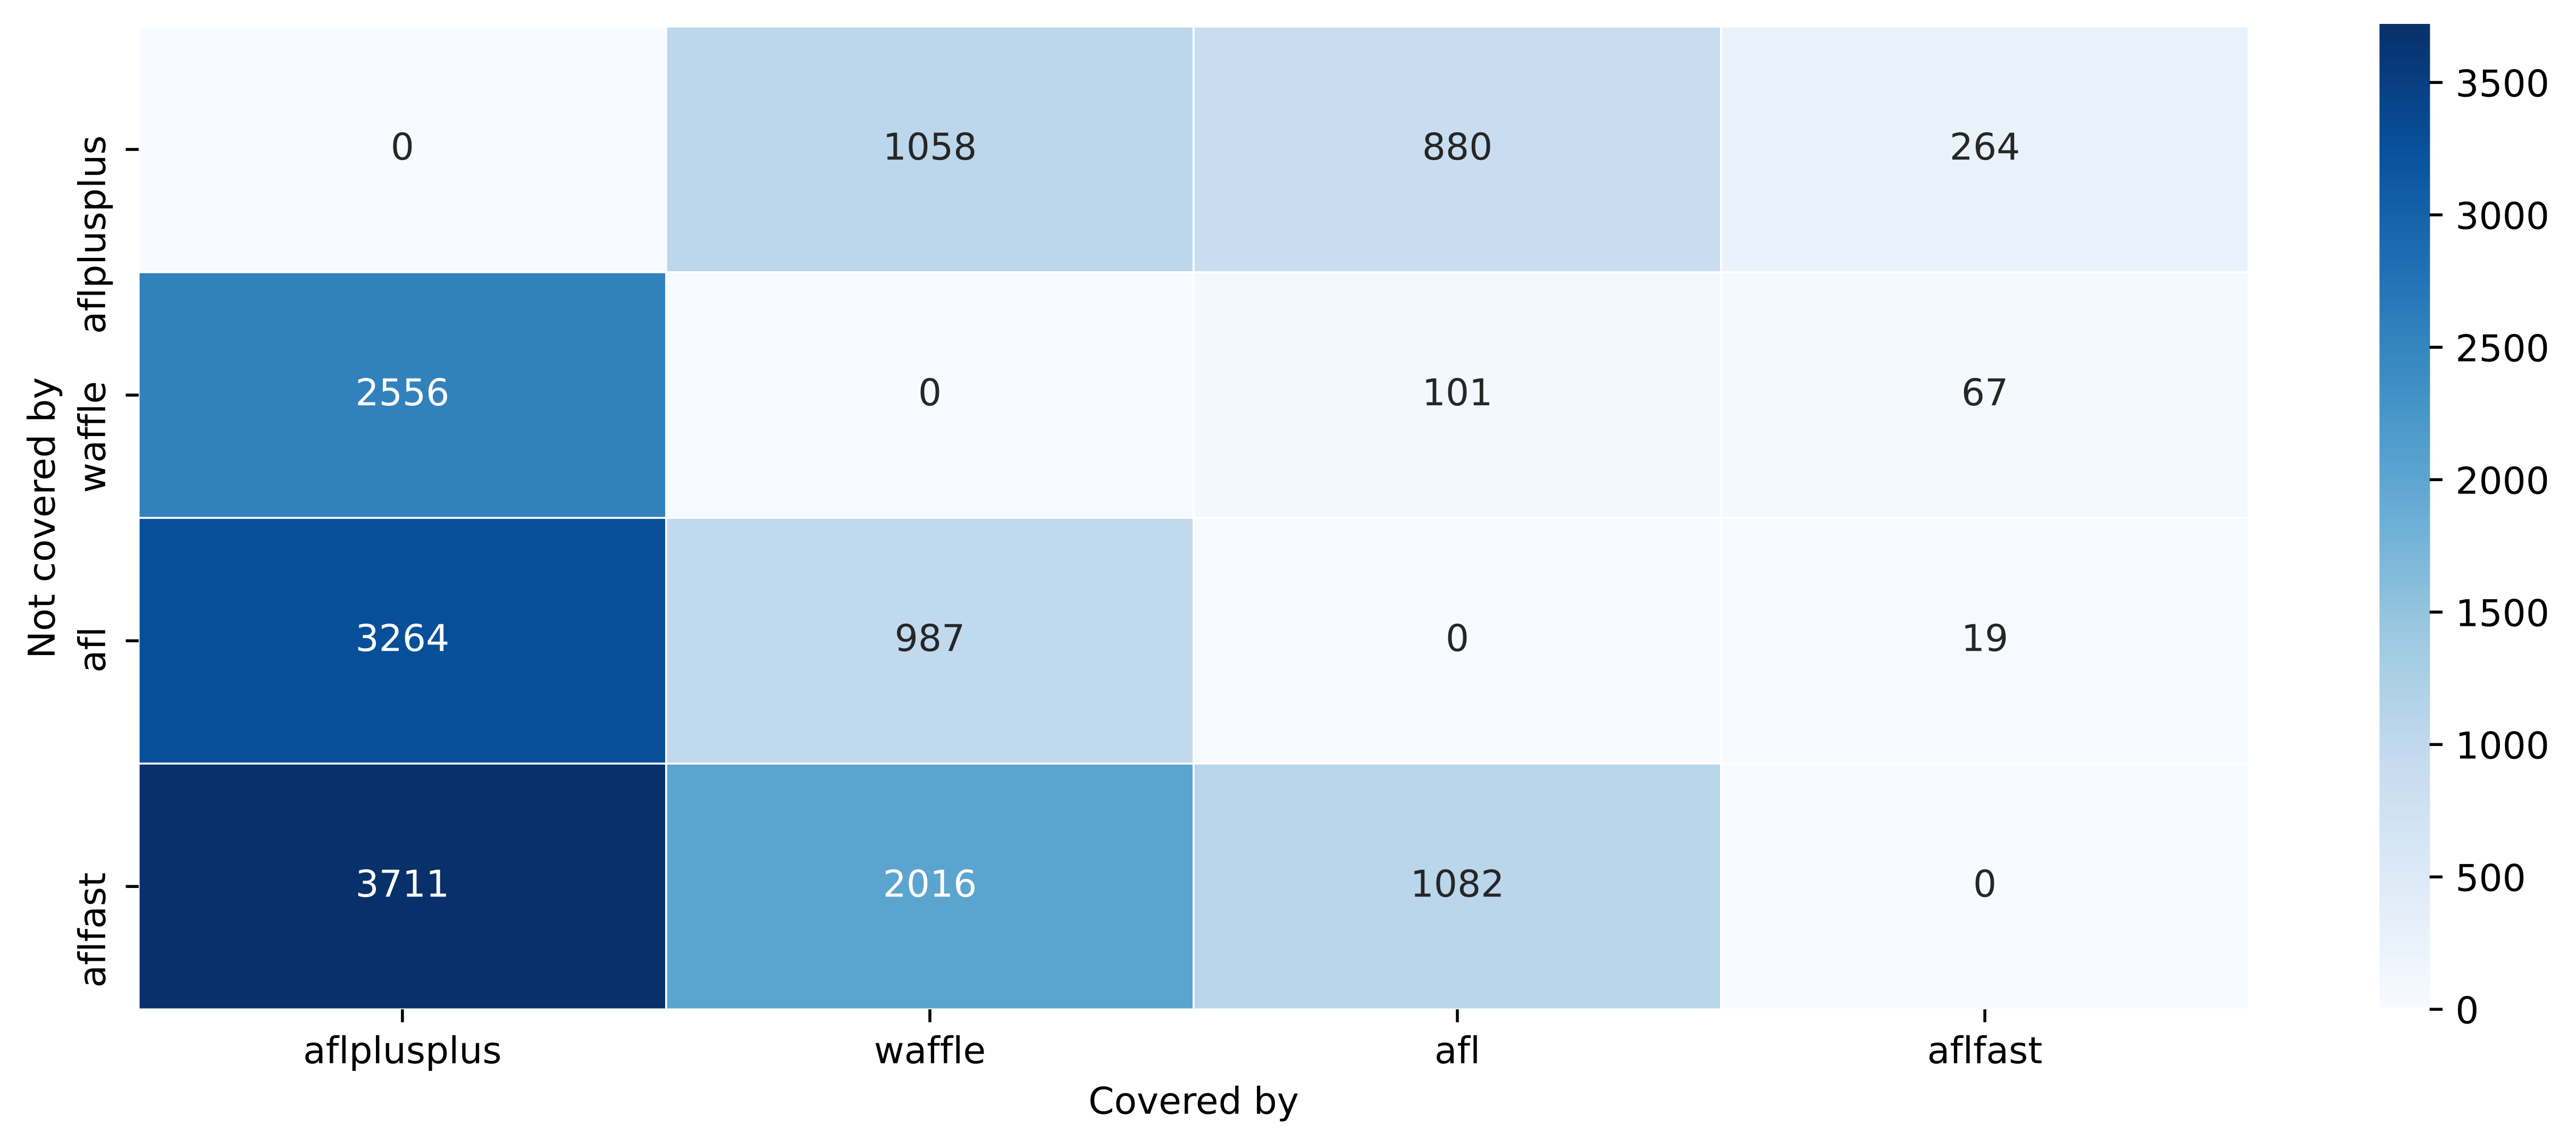
\includegraphics[width=0.70\textwidth]{Experiments/freetype2-2017_pairwise_unique_coverage_plot.png}
        \caption{freetype2-2017}
        \label{fig:sub:freetype-cov-uniq}
    \end{subfigure}

    \begin{subfigure}[t]{\textwidth}
        \centering
        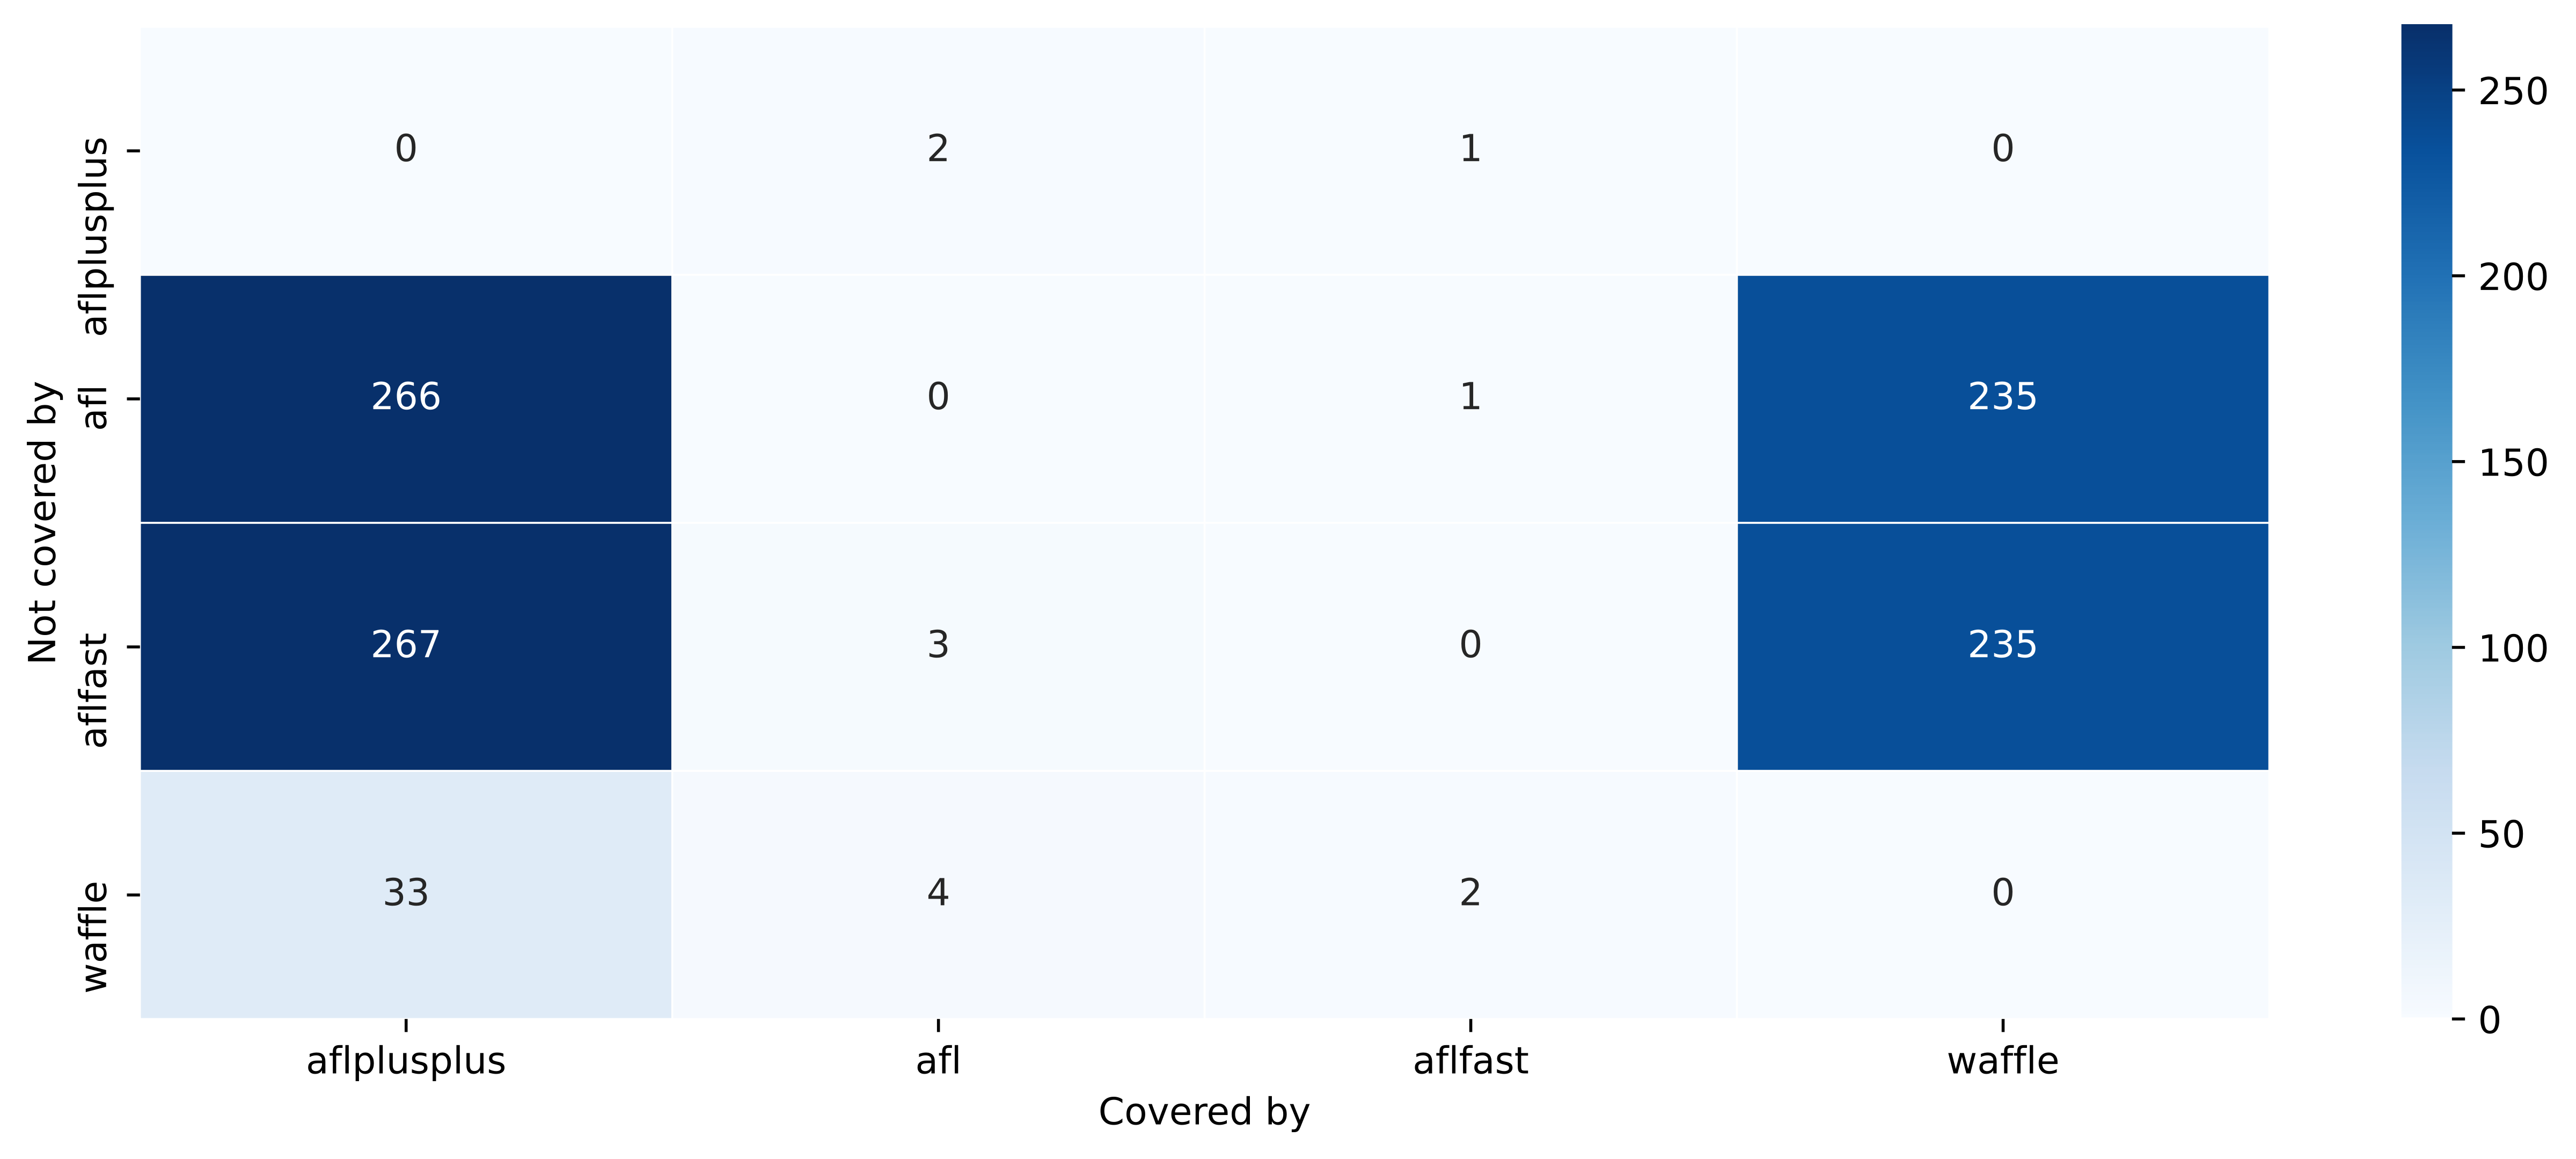
\includegraphics[width=0.70\textwidth]{Experiments/libjpeg-turbo-07-2017_pairwise_unique_coverage_plot.png}
        \caption{libjpeg-turbo-07-2017}
        \label{fig:sub:libjpeg-cov-uniq}
    \end{subfigure}

    \begin{subfigure}[t]{\textwidth}
        \centering
        \includegraphics[width=0.70\textwidth]{Experiments/libpng-1.2.56_pairwise_unique_coverage_plot.png}
        \caption{libpng-1.2.56}
        \label{fig:sub:libpng-cov-uniq}
    \end{subfigure}

    \begin{subfigure}[t]{\textwidth}
        \centering
        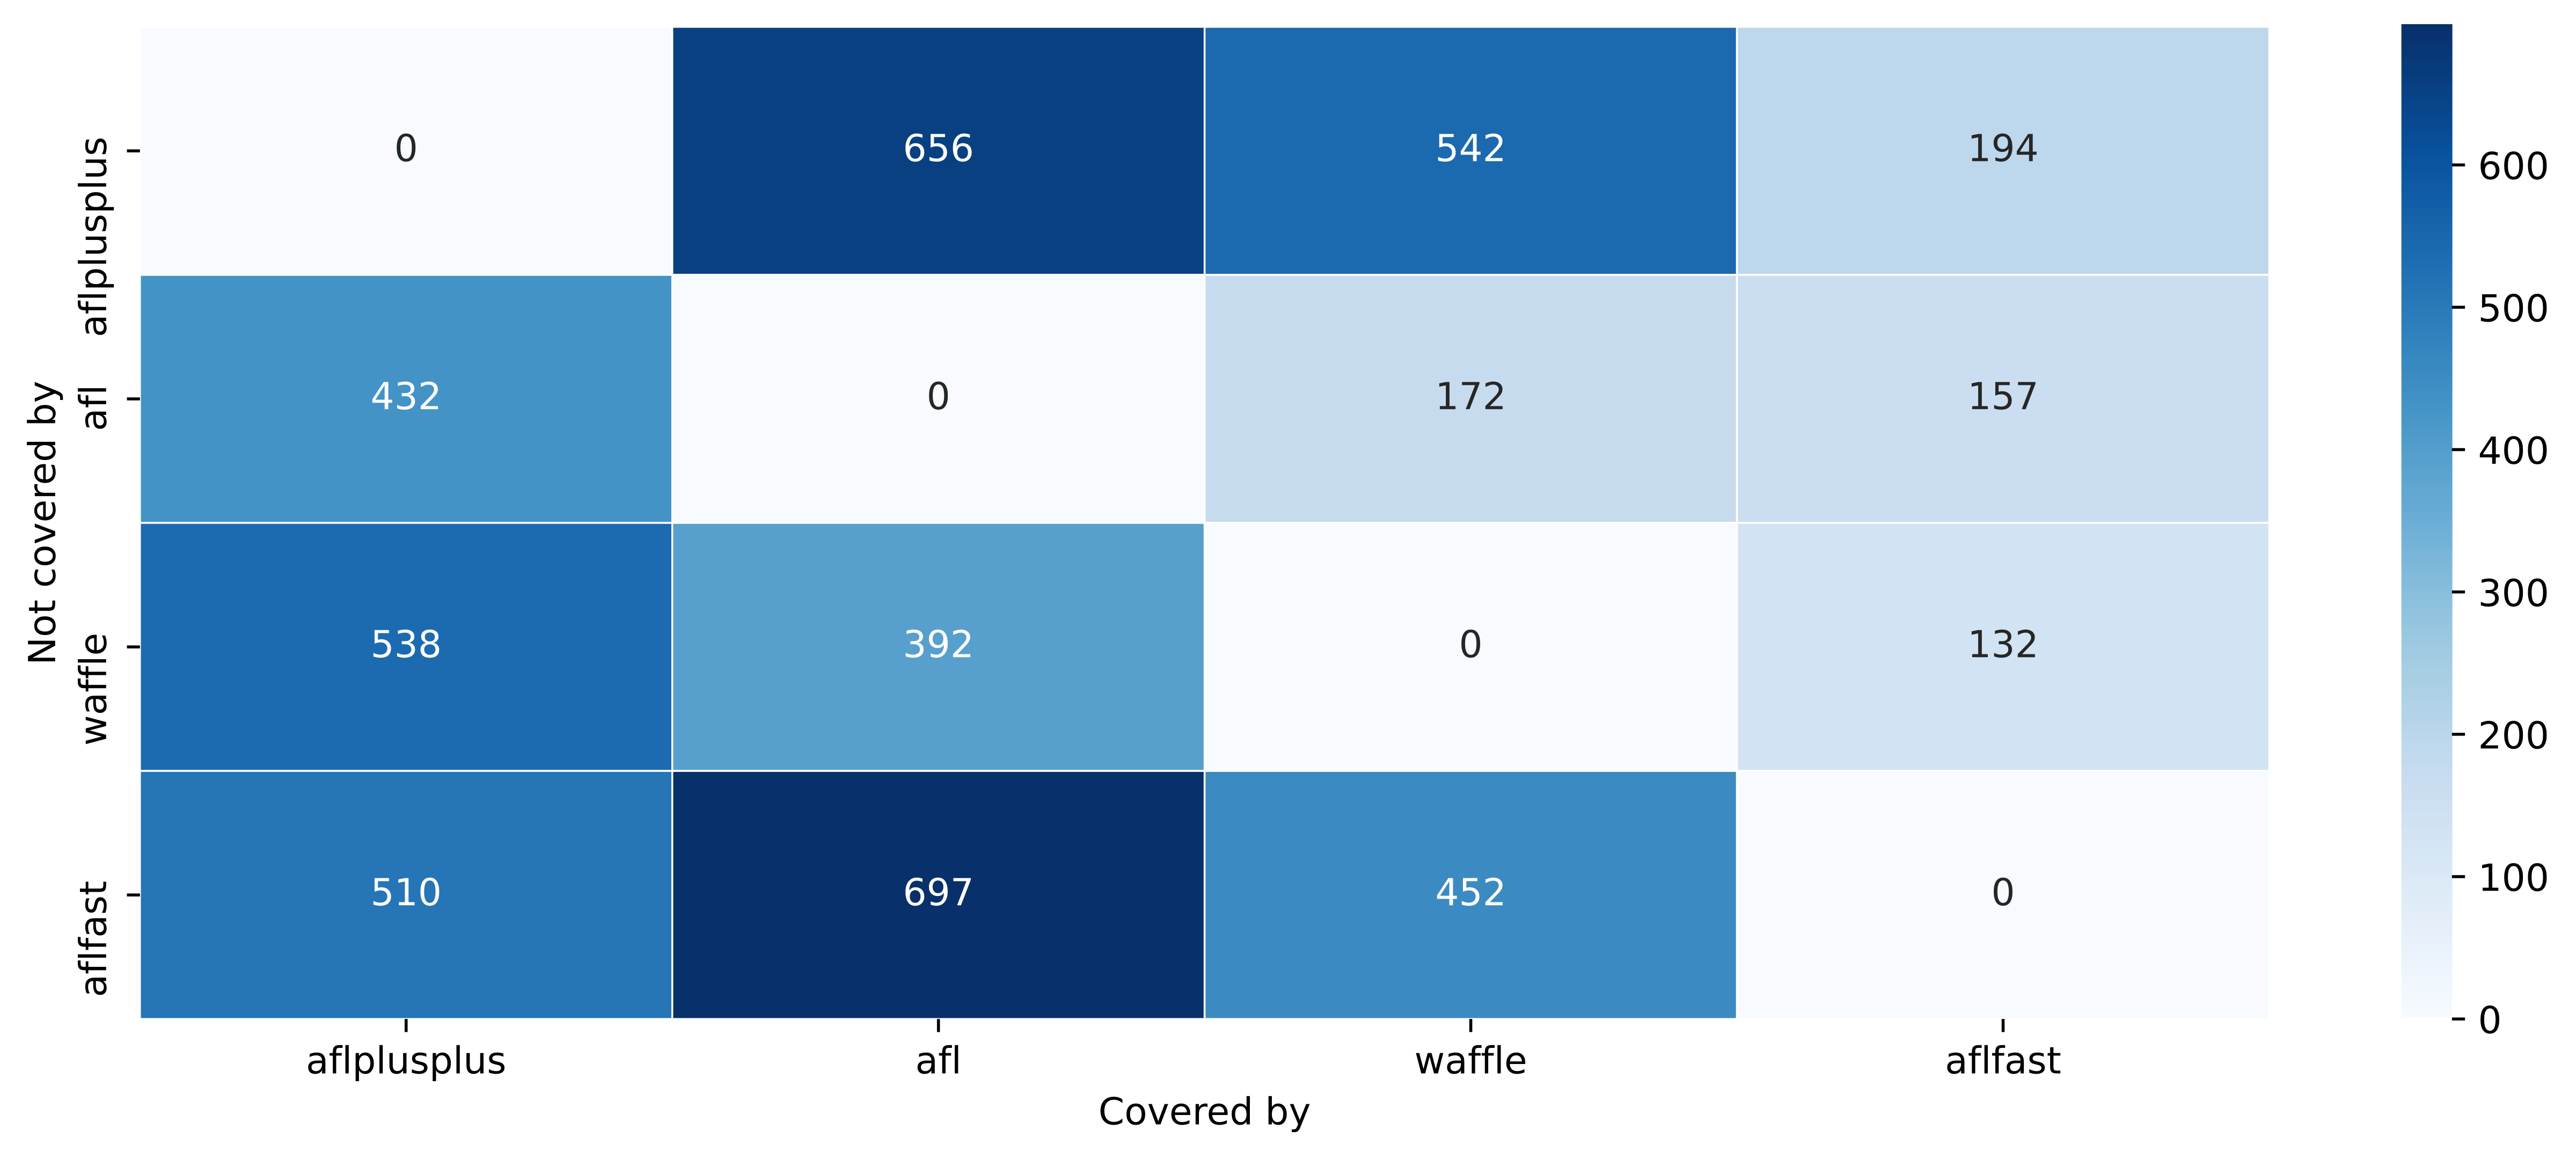
\includegraphics[width=0.70\textwidth]{Experiments/libxml2-v2.9.2_pairwise_unique_coverage_plot.png}
        \caption{libxml2-v2.9.2}
        \label{fig:sub:libxml-cov-uniq}
    \end{subfigure}

    \caption{Unique coverage findings}
    \label{fig:cov-growth-uniq}
\end{figure}


\begin{figure}
    \centering
    \begin{subfigure}[b]{0.475\linewidth}
        \centering
        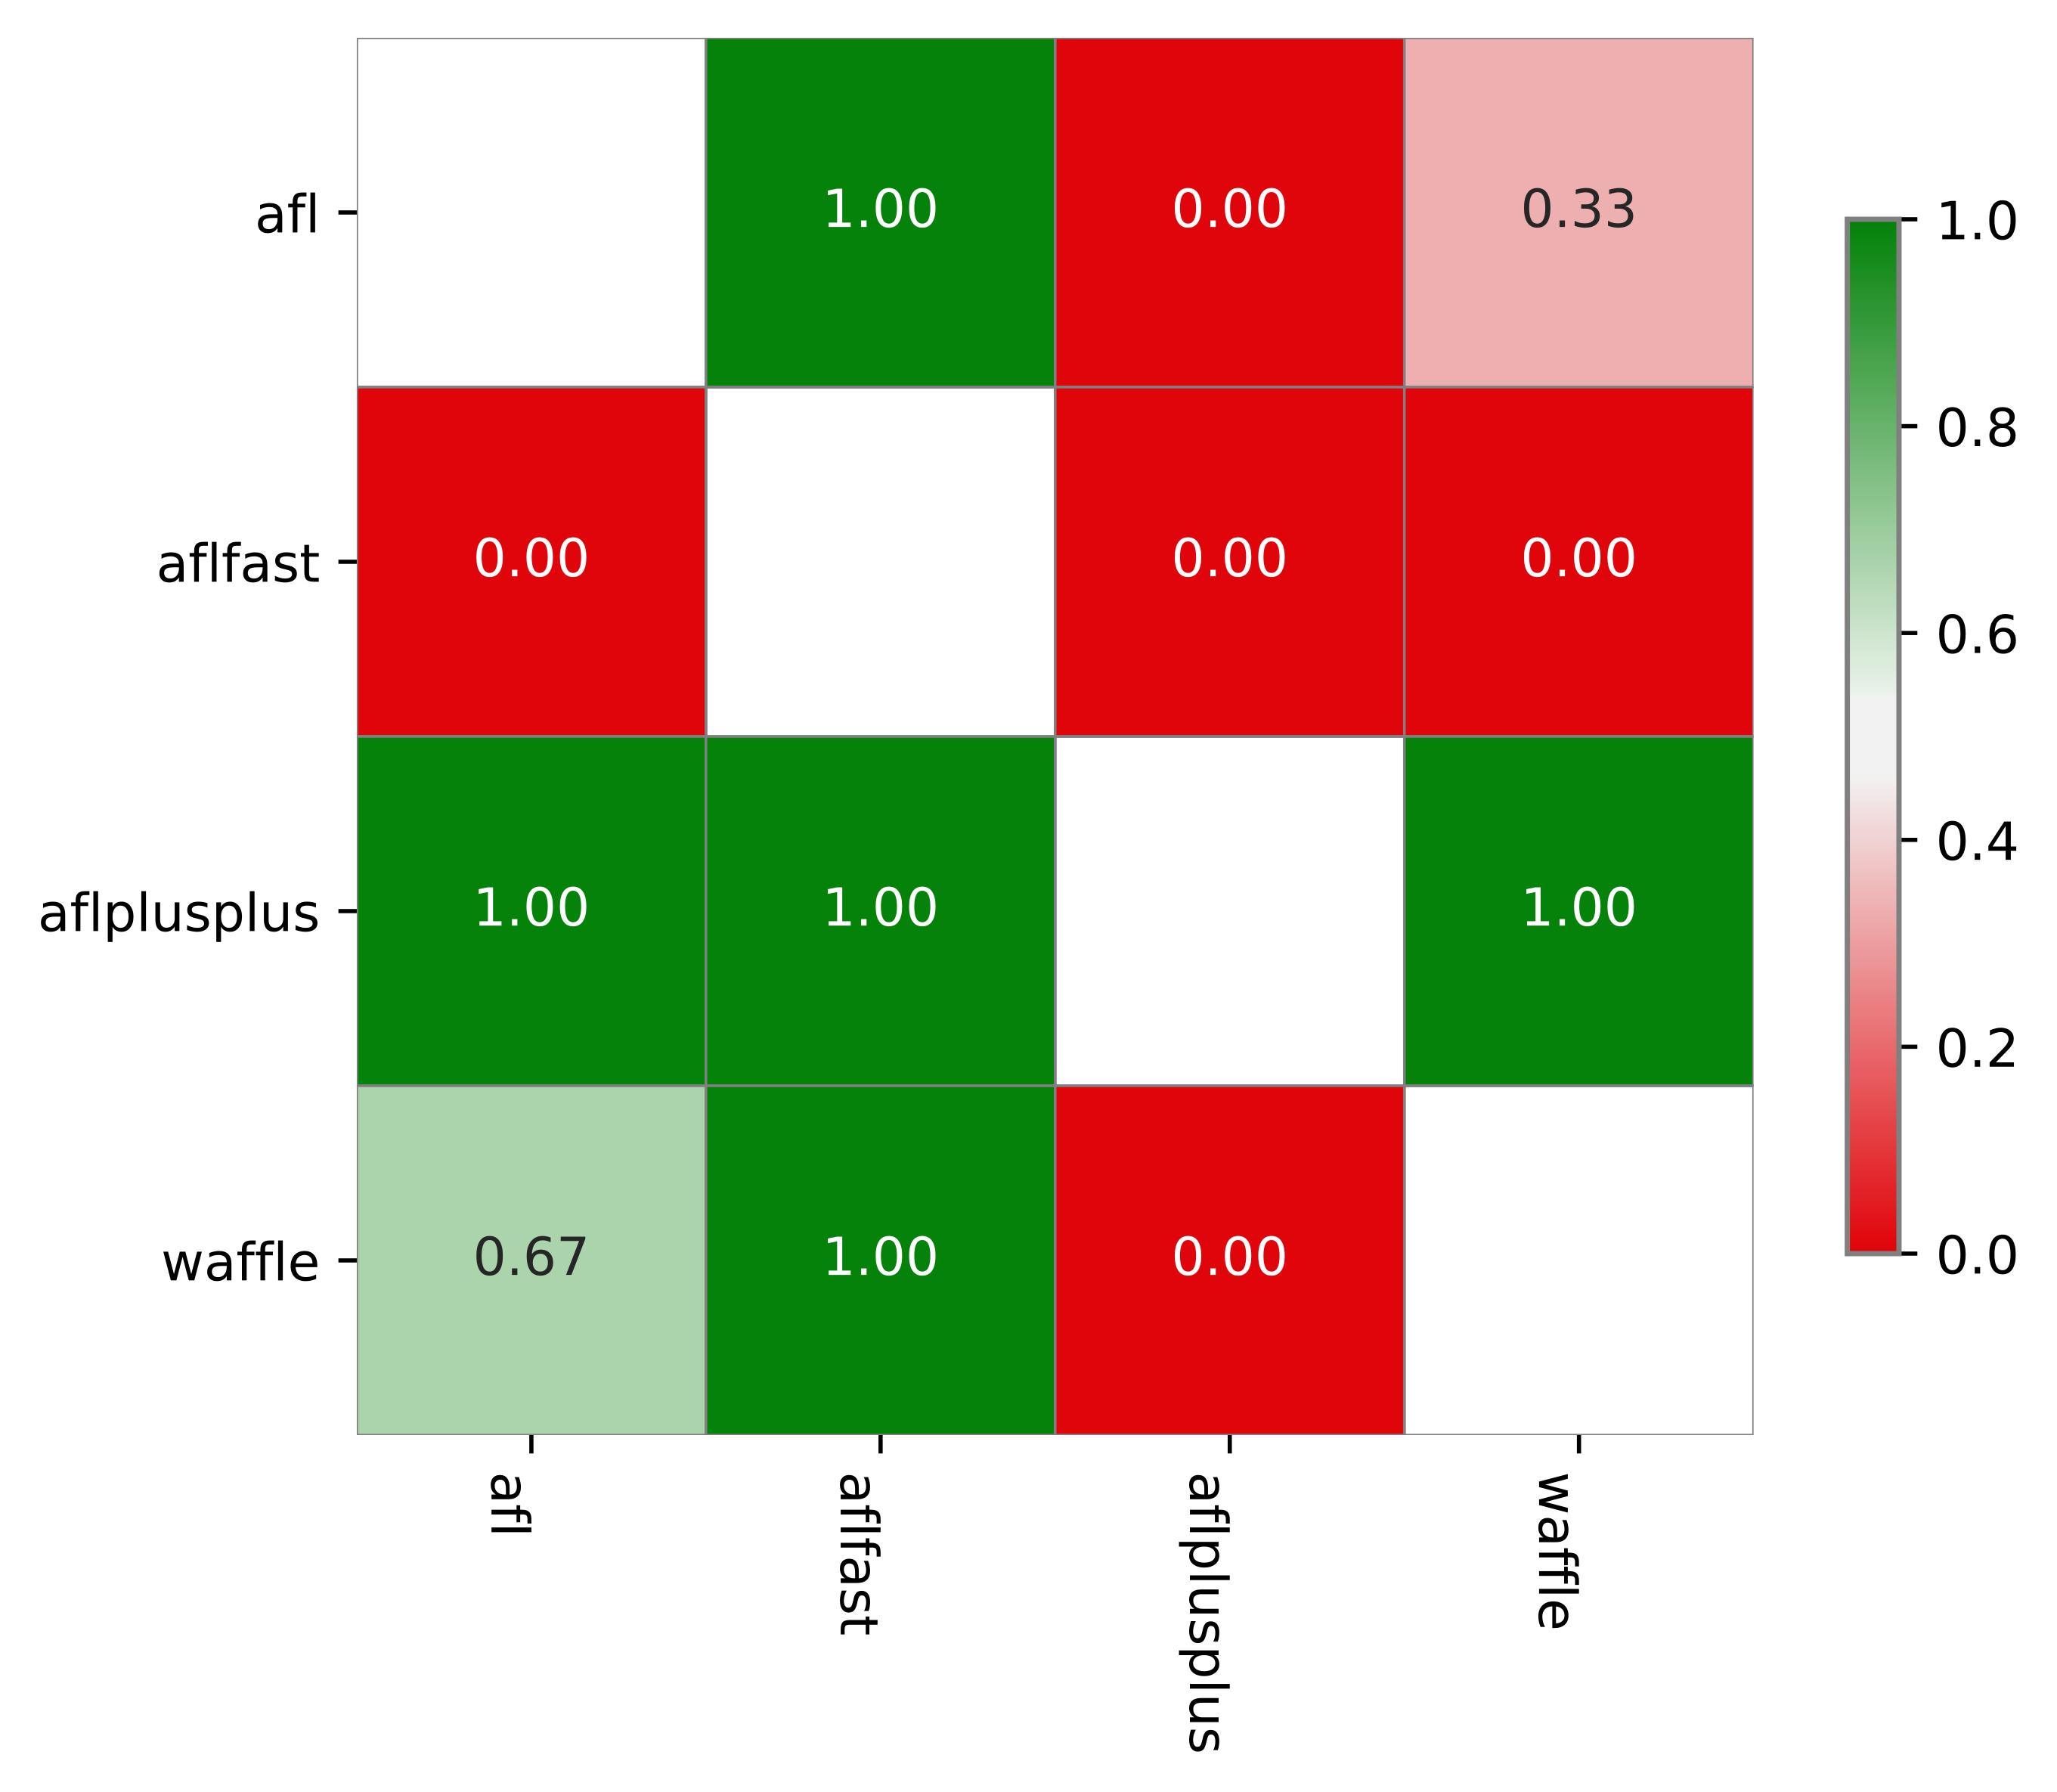
\includegraphics[width=0.95\linewidth]{Experiments/freetype2-2017_varga_delaney_a12_plot.png}
        \caption{freetype2-2017}
        \label{fig:sub:freetype-vda12}
    \end{subfigure}
    \begin{subfigure}[b]{0.475\linewidth}
        \centering
        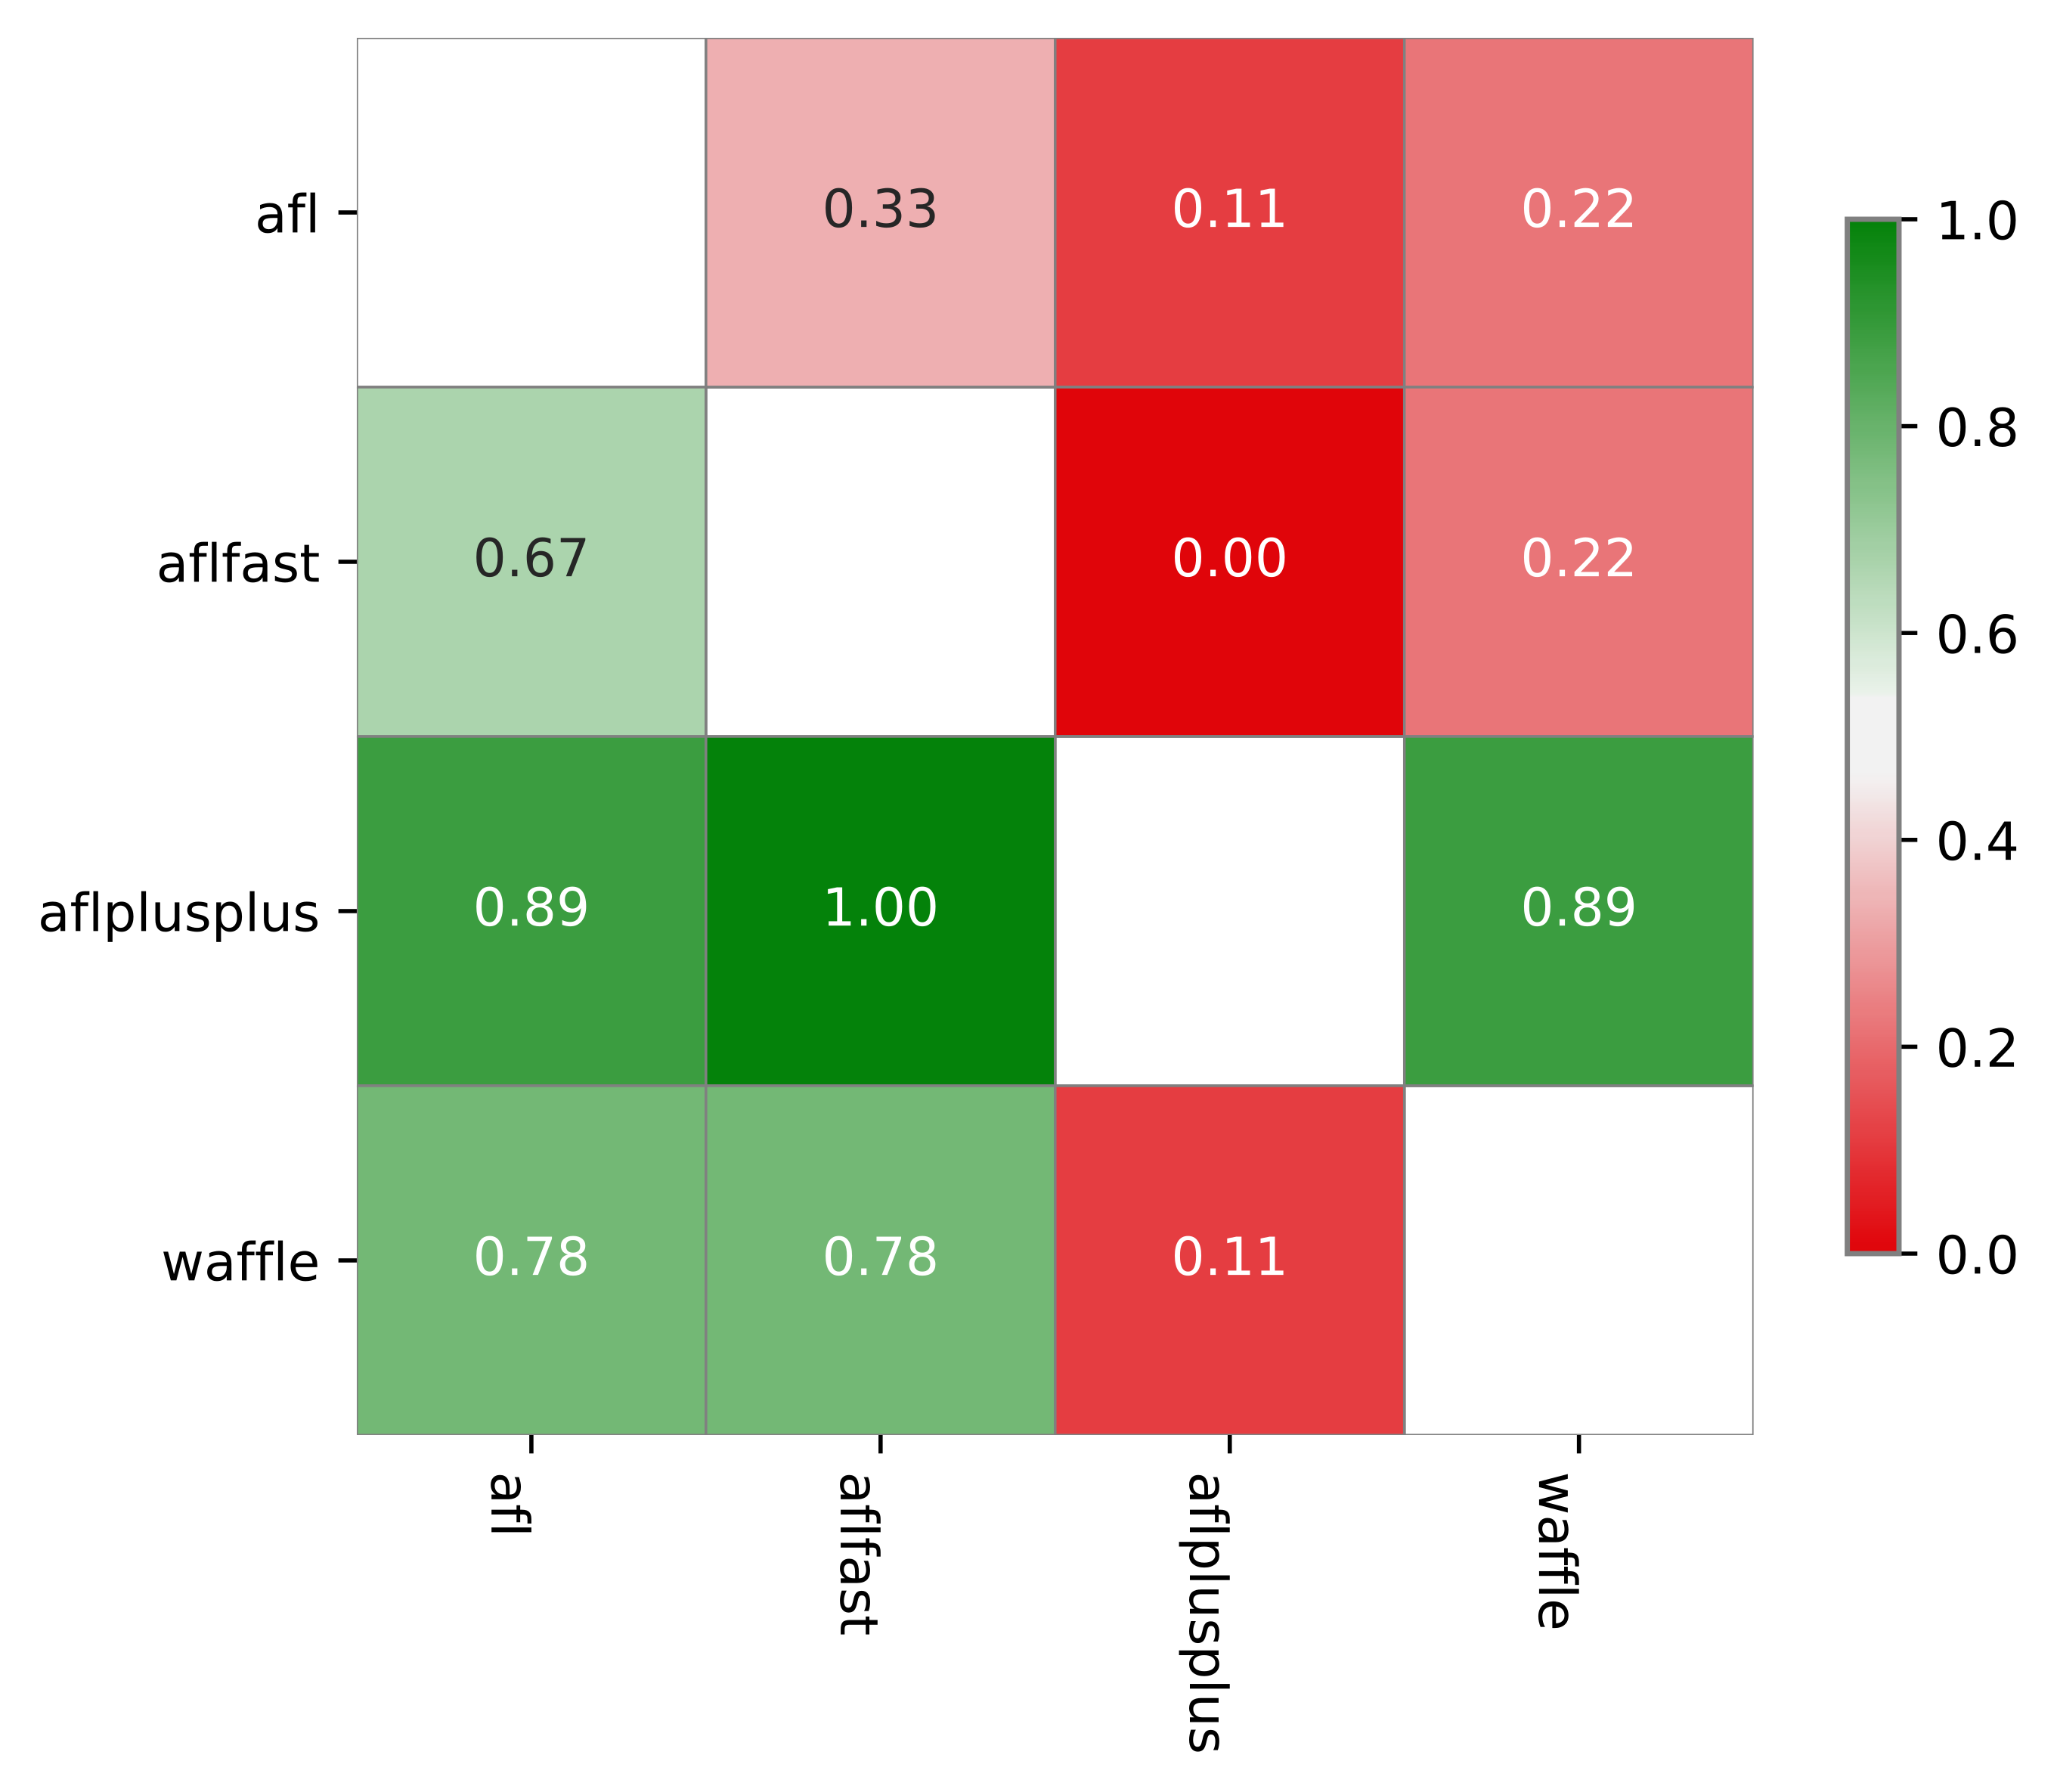
\includegraphics[width=0.95\linewidth]{Experiments/libjpeg-turbo-07-2017_varga_delaney_a12_plot.png}
        \caption{libjpeg-turbo-07-2017}
        \label{fig:sub:libjpeg-vda12}
    \end{subfigure}

    \begin{subfigure}[b]{0.475\linewidth}
        \centering
        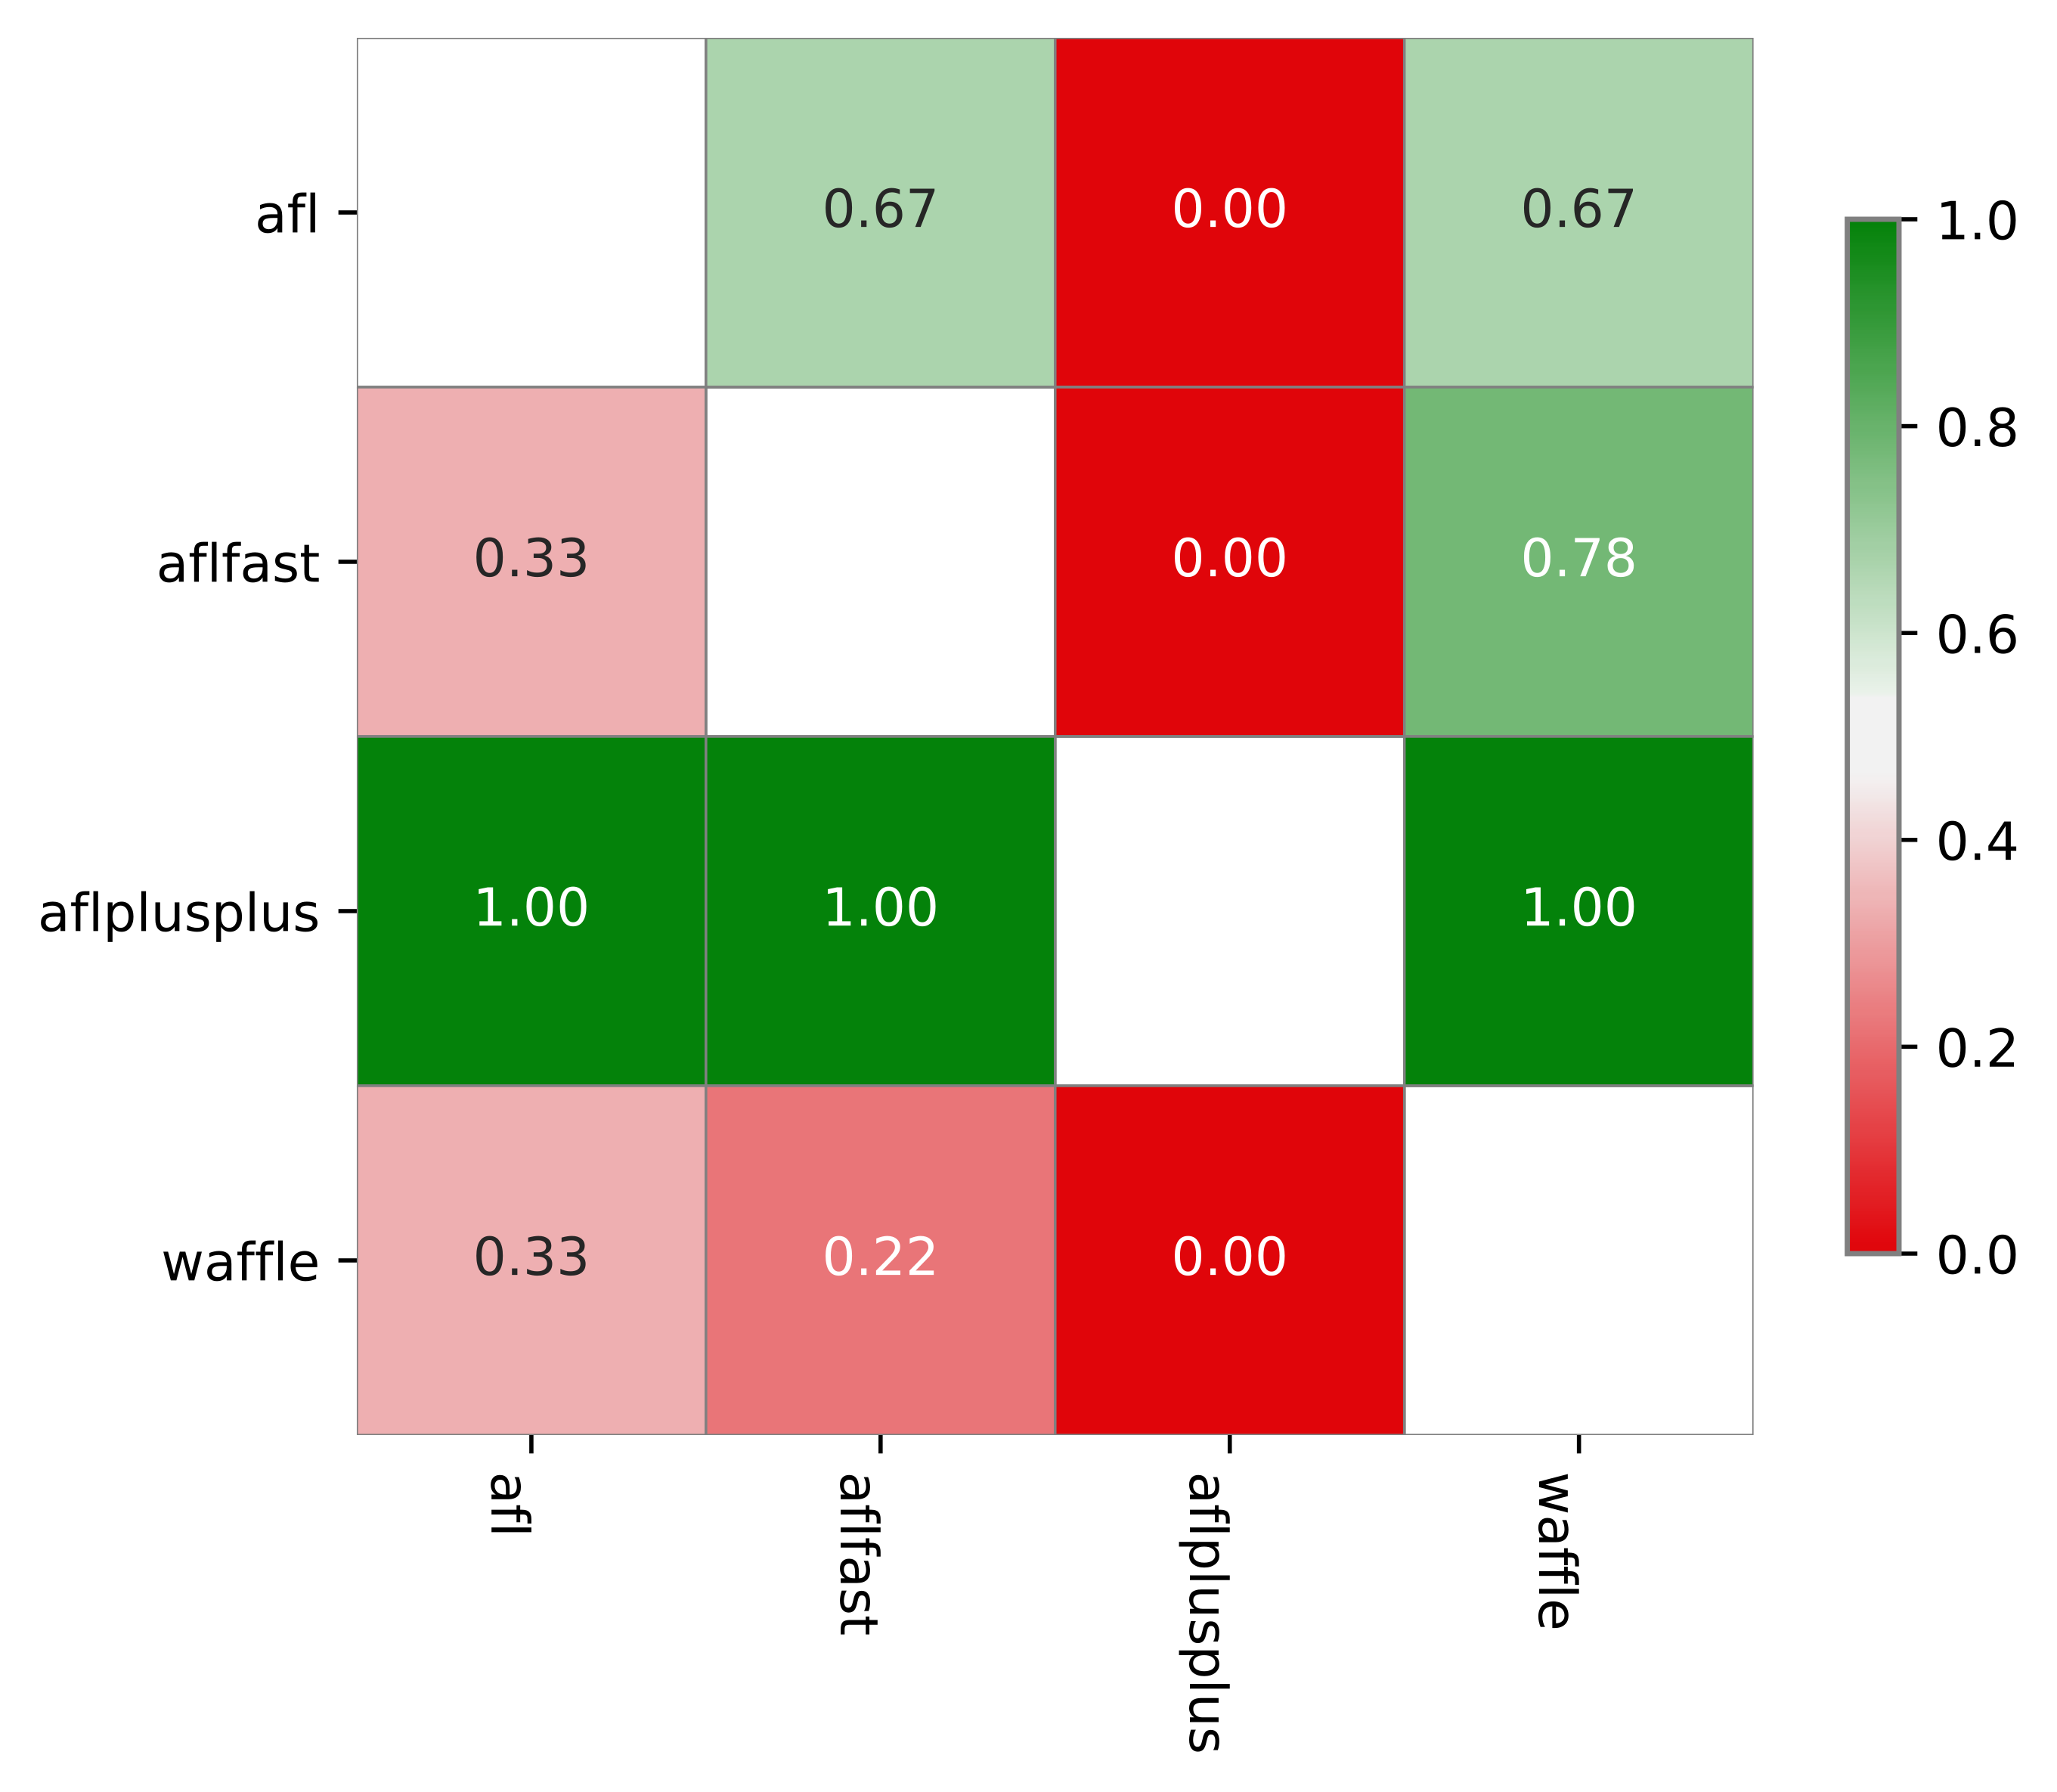
\includegraphics[width=0.95\linewidth]{Experiments/libpng-1.2.56_varga_delaney_a12_plot.png}
        \caption{libpng-1.2.56}
        \label{fig:sub:libpng-vda12}
    \end{subfigure}
    \begin{subfigure}[b]{0.475\linewidth}
        \centering
        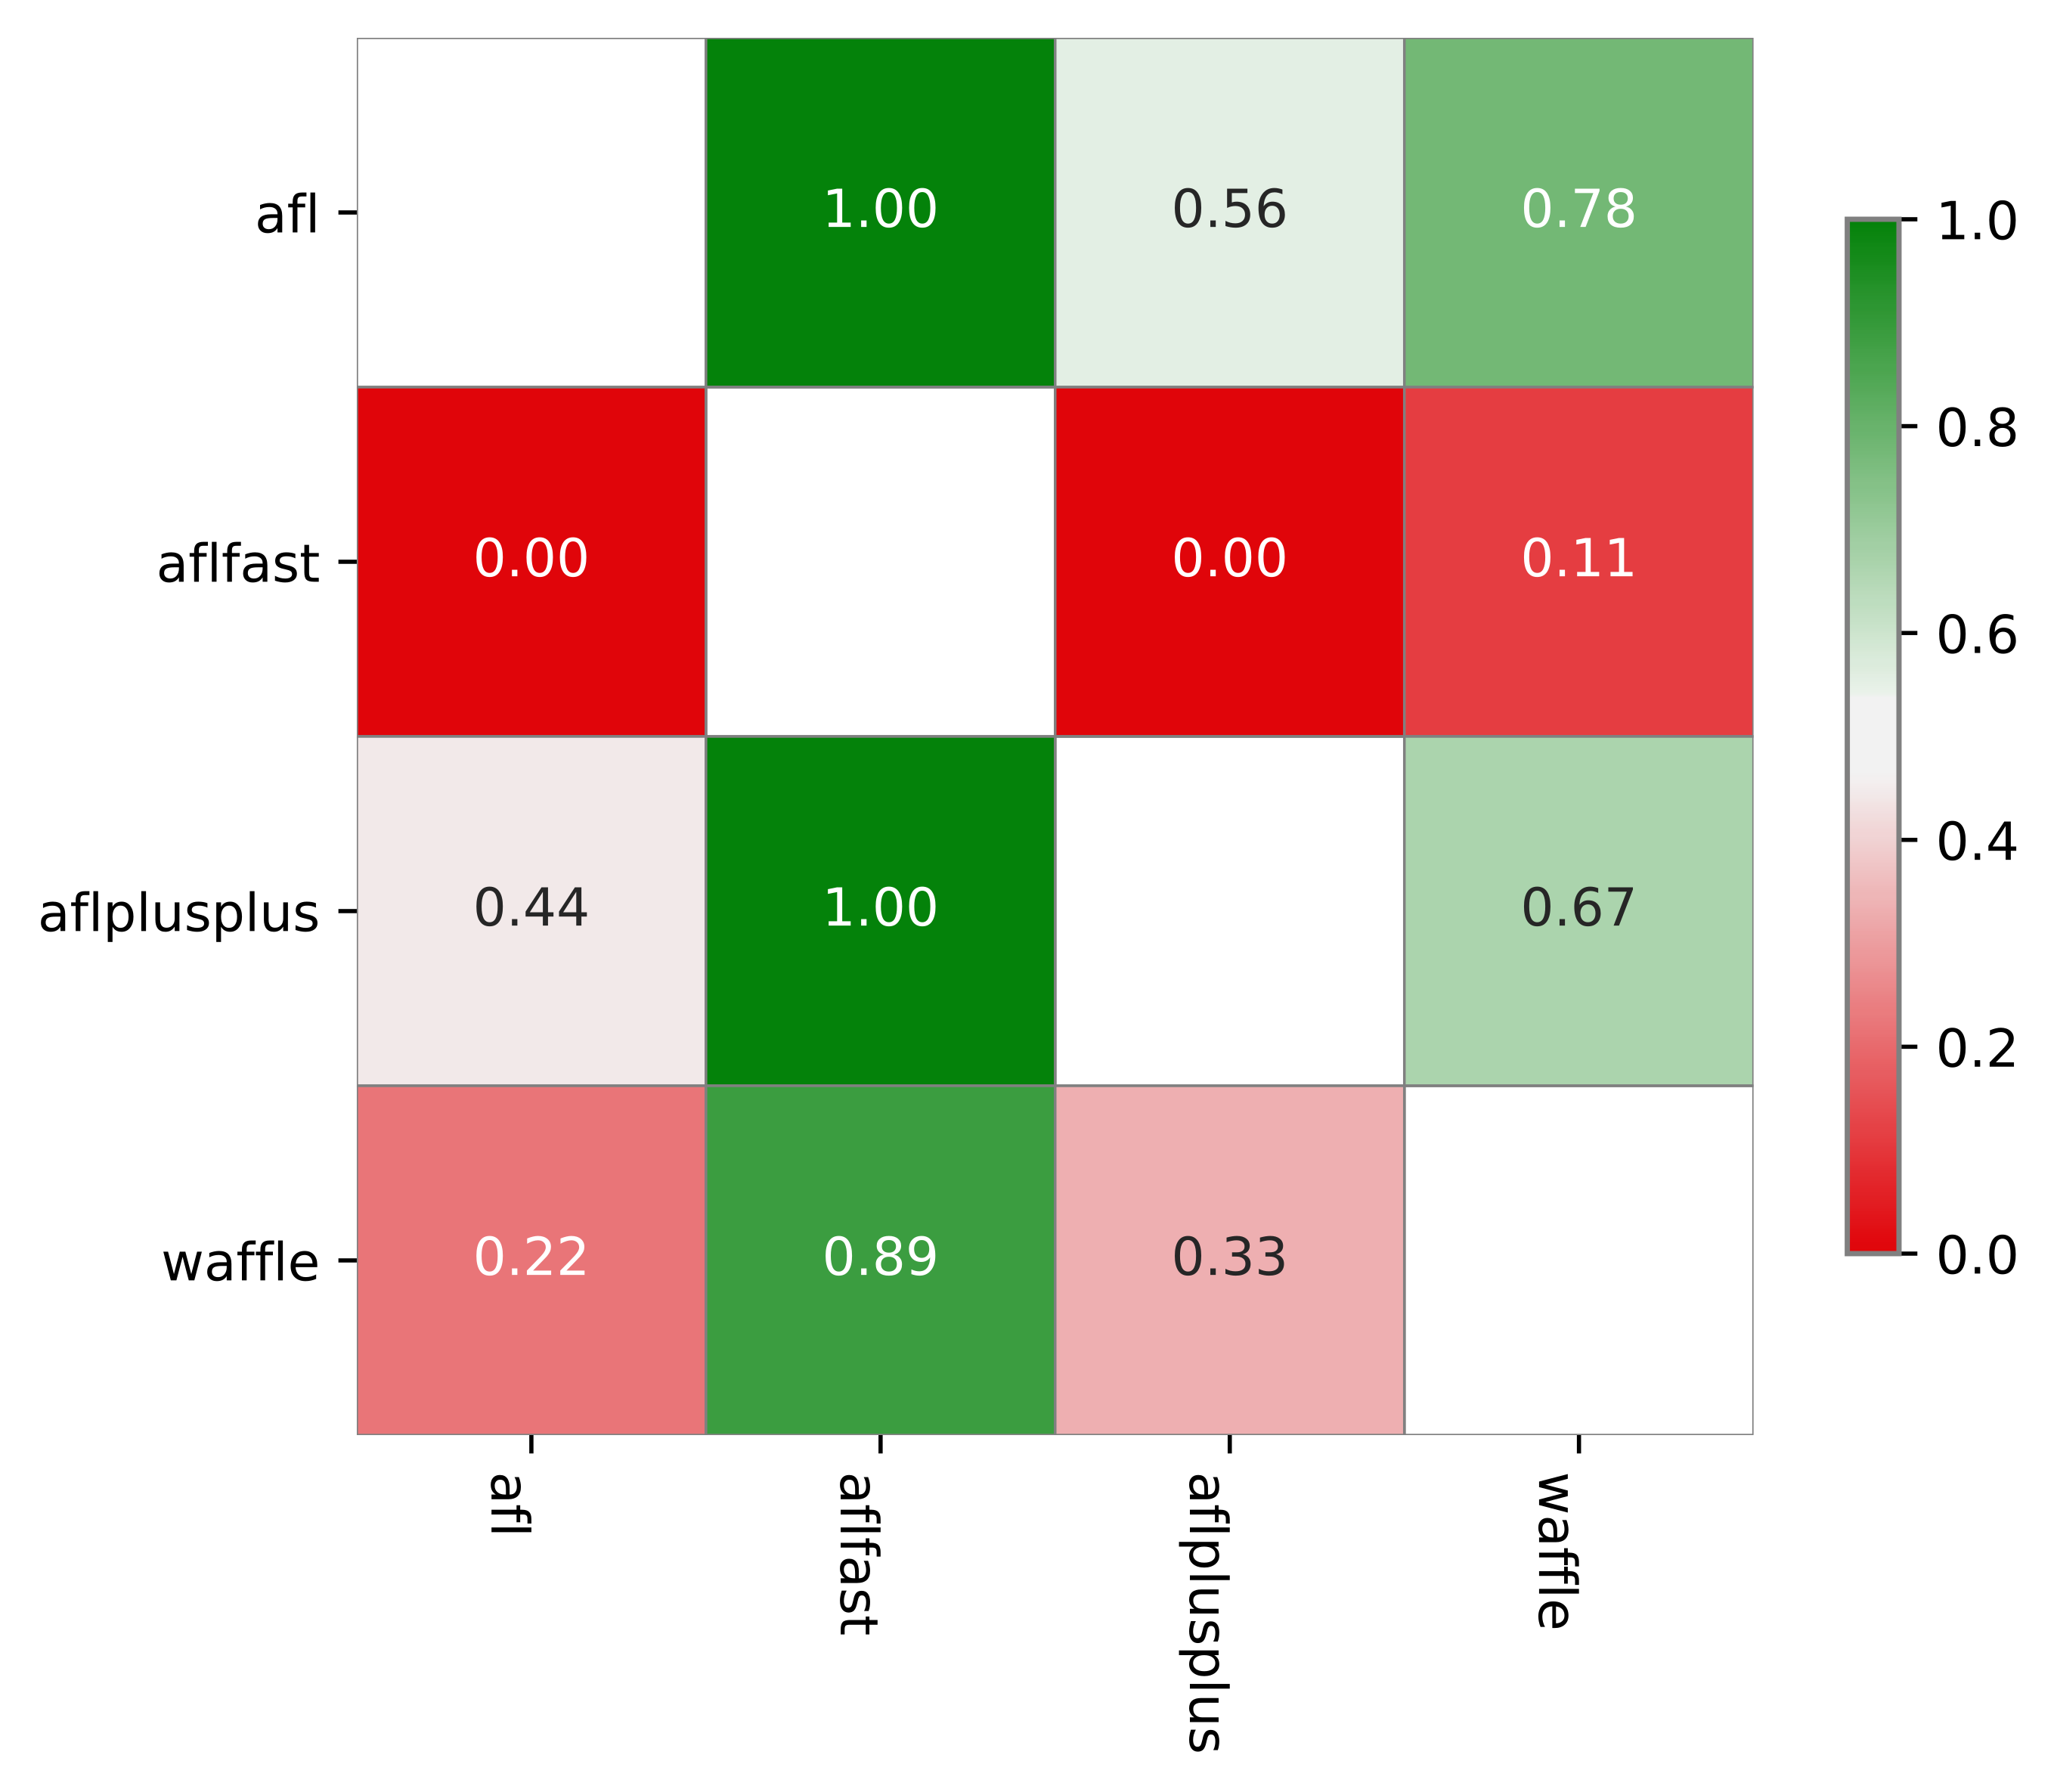
\includegraphics[width=0.95\linewidth]{Experiments/libxml2-v2.9.2_varga_delaney_a12_plot.png}
        \caption{libxml2-v2.9.2}
        \label{fig:sub:libxml-vda12}
    \end{subfigure}

    \caption{Unique coverage findings - The table summarizes the A12 values from the pairwise Vargha-Delaney A measure of effect size. Green cells indicate the probability the fuzzer in the row will outperform the fuzzer in the column.}
    \label{fig:vda12}
\end{figure}


FuzzBench starts reporting after building the project in a local experiment. Building AFL and Waffle on a benchmark such as \textit{libpng-1.2.56} took 30 minutes on the local computer, and FuzzBench doesn't generate any reports before that.

We tested Waffle in 6-hours experiments. The test computer could not run an experiment with more than \textbf{two fuzzers} and \textbf{one benchmark}, and the higher setups fail to finish. Each experiment contains \textbf{3} trials for each pair of $<FuzzerX, Benchmark>$, where FuzzerX is either Waffle, AFL, or LibFuzzer(LF). 

None of the trials could find any crashes/hangs during 6-hours trials.

Our experiments are:

\begin{enumerate}
    \item Waffle vs AFL on libpng-1.2.56
    \item Waffle vs LibFuzzer on libpng-1.2.56
    \item Waffle vs AFL on openthread-2019-12-23
    \item Waffle vs LibFuzzer on openthread-2019-12-23
    \item Waffle vs AFL on php\_php-fuzz-execute
    \item Waffle vs LibFuzzer on php\_php-fuzz-execute
    \item Waffle vs AFL on curl\_curl\_fuzzer\_http
    \item Waffle vs AFL on sqlite3\_ossfuzz
\end{enumerate}

We evaluate the results according to the generated reports. The graphs [Figures \ref{fig:report-log}, \ref{fig:report-box}, and \ref{fig:report-unq}] illustrate the covered regions of the code in each experiment, the pairwise unique coverage, and the growth of the code coverage over time. Green color represents Waffle in all figures.



For the benchmarks \textit{libpng-1.2.56}, \textit{php\_php-fuzz-execute}, and \textit{openthread}, we analyzed the performance of Waffle with each on of the other fuzzers. In our setups, we continued testing \textit{sqlite3\_ossfuzz} and \textit{curl\_curl\_fuzzer\_http} with Waffle and AFL for further investigations.

\subsection*{Performance measurements}

FuzzBench compares the performance of the fuzzers based on the discovered code coverage of each experiment. Meaning that, for example, FuzzBench does not check how many executions a fuzzer performs; instead, it considers the variety of the generated inputs, according to their execution paths. 

Table \ref{table:all} shows the summary of our results. The table shows the coverage stats for the participating fuzzers; the columns are $mean coverage$, $standard deviation$, and the number of $unique findings$ of each fuzzer in each experiment.

\begin{table}[!t]
    \begin{adjustbox}{angle=90}
        {\setlength{\extrarowheight}{2ex}%
        \begin{tabular}{|l|c|c|c|c|c|c|} 
        \hline
        \textbf{Benchmark}                & \textbf{Fuzzer}    & \begin{tabular}[c]{@{}c@{}}\textbf{Waffle}\\ \textbf{Mean Coverage}\end{tabular} & \begin{tabular}[c]{@{}c@{}}\textbf{Fuzzer}\\ \textbf{Mean Coverage}\end{tabular} & \begin{tabular}[c]{@{}c@{}}\textbf{Waffle}\\ \textbf{STD}\end{tabular} & \begin{tabular}[c]{@{}c@{}}\textbf{Fuzzer}\\ \textbf{STD}\end{tabular} & \begin{tabular}[c]{@{}c@{}}\textbf{Unique}\\ \textbf{(Waffle/Fuzzer)}\end{tabular}  \\[2ex] 
        \hline
        libpng-1.2.56            & AFL       & 1509                                                           & 1510                                                           & 0.57                                                 & 0.57                                                 & 0/1                                                               \\[2ex] 
        \hline
        libpng-1.2.56            & LibFuzzer & 1509                                                           & 1951                                                           & 0.57                                                 & 6.65                                                 & 0/425                                                             \\[2ex]
        \hline
        php\_php-fuzz-execute    & AFL       & 147945                                                         & 169447                                                         & 5451.77                                              & 2069.34                                              & 1270/18902                                                        \\[2ex]
        \hline
        php\_php-fuzz-execute    & LibFuzzer & 145816                                                         & 138666                                                         & 2580.20                                              & 234.08                                               & 10179/335                                                         \\[2ex] 
        \hline
        openthread-2019-12-23    & AFL       & 5226                                                           & 5216                                                           & 12.58                                                & 24.13                                                & 0/2                                                               \\[2ex]
        \hline
        openthread-2019-12-23    & LibFuzzer & 5242                                                           & 5852                                                           & 3.21                                                 & 24.24                                                & 6/384                                                             \\[2ex]
        \hline
        sqlite3\_ossfuzz         & AFL       & 33510                                                          & 32245                                                          & 2631.01                                              & 872.98                                               & 1435/1088                                                         \\[2ex]
        \hline
        curl\_curl\_fuzzer\_http & AFL       & 17142                                                          & 17290                                                          & 215.89                                               & 192.12                                               & 55/154                                                            \\[2ex]
        \hline
        \end{tabular}}
    \end{adjustbox}
    \caption{Statistics of the experiments.}
    \label{table:all}
\end{table}

Figure \ref{fig:report-log} shows the growth of the code coverage that each fuzzer had explored. In testing \textit{libpng} [\ref{gro:b}], \textit{openthread} [\ref{gro:e}], and \textit{curl} [\ref{gro:a}], we can see that both Waffle and AFL eventually converge, and it suggests that, here, Waffle performs indifferently in the discovery of new regions of code (higher code coverage). Waffle also shows latency in generating the first generations of the inputs and continues a close competition with AFL.

For \textit{php\_php-fuzz-execute}, AFL shows 15\% better performance; however, for the other benchmark, \textit{sqlite3\_ossfuzz}, Waffle has enhanced the performance of AFL by 4\%.

LibFuzzer is showing better performance than Waffle as in Figures \ref{gro:f} and \ref{gro:h}. LibFuzzer found 30\% and 12\% more code coverage for fuzzing \textit{libpng} and \textit{openthread}, respectively. On the other hand, fuzzing \textit{php} has 5\% more code coverage under Waffle.

Comparing the graphs on the left column (AFL) and the right column (LF) for the benchmarks, \textit{libpng}, \textit{openthread}, and \textit{php}, shows the following rankings:

\begin{enumerate}
    \item \textbf{libpng:} 1: LibFuzzer. 2: Waffle/AFL.
    \item \textbf{openthread:} 1: LibFuzzer. 2: Waffle/AFL.
    \item \textbf{php:} 1: AFL. 2: Waffle. 3: LibFuzzer.
\end{enumerate}

In the third scenario, we see that in the \textit{6-hours} trials, Waffle succeeds LibFuzzer for fuzzing \textit{php}.

\begin{figure}[!t]
    \begin{adjustbox}{center,max width=1.3\textwidth}
        \begin{subfigure}[t]{0.55\textwidth}
            \centering
            \includegraphics[width=\textwidth]{Chapter4/experimental/WA-lib/libpng-1.2.56_coverage_growth.png}
            \vspace*{-5mm}
            \caption{Waffle-AFL libpng-1.2.56}
            \label{gro:b}
            \vspace*{5mm}
        \end{subfigure}
        ~
        \begin{subfigure}[t]{0.55\textwidth}
            \centering
            \includegraphics[width=\textwidth]{Chapter4/experimental/WL-lib/libpng-1.2.56_coverage_growth.png}
            \vspace*{-5mm}
            \caption{Waffle-LF libpng-1.2.56}
            \label{gro:f}
            \vspace*{5mm}
        \end{subfigure}
    \end{adjustbox}
    ~
    \begin{adjustbox}{center,max width=1.3\textwidth}
        \begin{subfigure}[t]{0.55\textwidth}
            \centering
            \includegraphics[width=\textwidth]{Chapter4/experimental/WA-thr/openthread-2019-12-23_coverage_growth.png}
            \vspace*{-5mm}
            \caption{Waffle-AFL openthread-2019-12-23}
            \label{gro:e}
            \vspace*{5mm}
        \end{subfigure}
        ~
        \begin{subfigure}[t]{0.55\textwidth}
            \centering
            \includegraphics[width=\textwidth]{Chapter4/experimental/WL-thr/openthread-2019-12-23_coverage_growth.png}
            \vspace*{-5mm}
            \caption{Waffle-LF openthread-2019-12-23}
            \label{gro:h}
            \vspace*{5mm}
        \end{subfigure}
    \end{adjustbox}
    ~
    \begin{adjustbox}{center,max width=1.3\textwidth}
        \begin{subfigure}[t]{0.55\textwidth}
            \centering
            \includegraphics[width=\textwidth]{Chapter4/experimental/WA-php/php_php-fuzz-execute_coverage_growth.png}
            \vspace*{-5mm}
            \caption{Waffle-AFL php\_php-fuzz-execute}
            \label{gro:c}
            \vspace*{5mm}
        \end{subfigure}
        ~
        \begin{subfigure}[t]{0.55\textwidth}
            \centering
            \includegraphics[width=\textwidth]{Chapter4/experimental/WL-php/php_php-fuzz-execute_coverage_growth.png}
            \vspace*{-5mm}
            \caption{Waffle-LF php\_php-fuzz-execute}
            \label{gro:g}
            \vspace*{5mm}
        \end{subfigure}
    \end{adjustbox}
    ~
    \begin{adjustbox}{center,max width=1.3\textwidth}
        \begin{subfigure}[t]{0.55\textwidth}
            \centering
            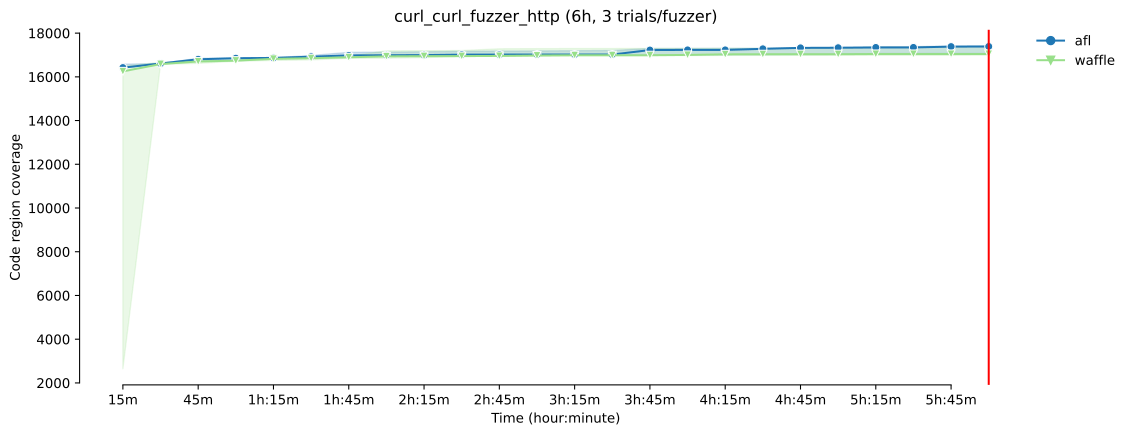
\includegraphics[width=\textwidth]{Chapter4/experimental/WA-cur/curl_curl_fuzzer_http_coverage_growth.png}
            \vspace*{-5mm}
            \caption{Waffle-AFL curl\_curl\_fuzzer\_http}
            \label{gro:a}
            \vspace*{5mm}
        \end{subfigure}
        ~
        \begin{subfigure}[t]{0.55\textwidth}
            \centering
            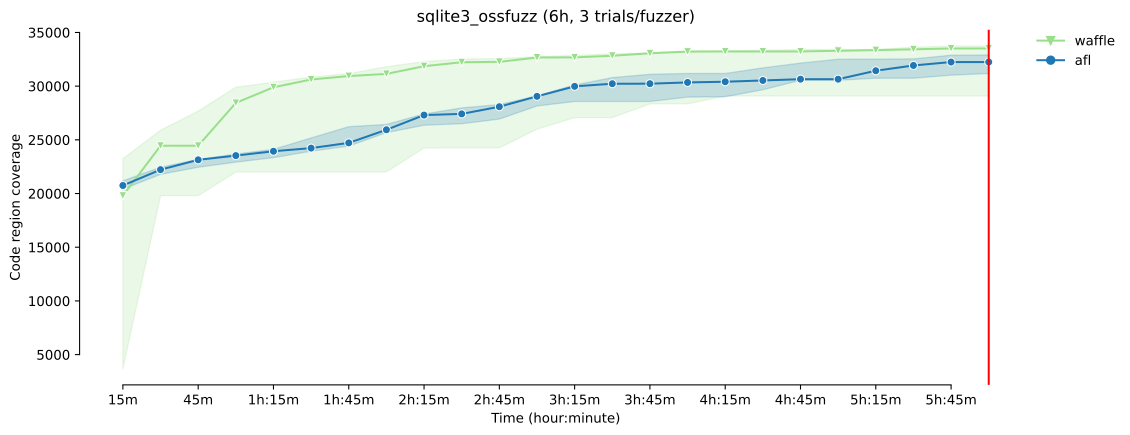
\includegraphics[width=\textwidth]{Chapter4/experimental/WA-sql/sqlite3_ossfuzz_coverage_growth.png}
            \vspace*{-5mm}
            \caption{Waffle-AFL sqlite3\_ossfuzz}
            \label{gro:d}
            \vspace*{5mm}
        \end{subfigure}
    \end{adjustbox}
    \caption{Mean code coverage growth over time}
    \label{fig:report-log}
\end{figure}

In Figure \ref{fig:report-box}, we can analyze the distribution of the code-coverages of each trial pair. The code coverage of AFL shows lower deviations compared to Waffle.

\begin{figure}[!t]
    \begin{adjustbox}{center,max width=1.3\textwidth}
        \begin{subfigure}[t]{0.5\textwidth}
            \centering
            \includegraphics[width=\textwidth]{Chapter4/experimental/WA-lib/libpng-1.2.56_boxplot.png}
            \vspace*{-5mm}
            \caption{Waffle-AFL libpng-1.2.56}
            \label{box:wal}
            \vspace*{5mm}
        \end{subfigure}
        ~
        \begin{subfigure}[t]{0.5\textwidth}
            \centering
            \includegraphics[width=\textwidth]{Chapter4/experimental/WL-lib/libpng-1.2.56_boxplot.png}
            \vspace*{-5mm}
            \caption{Waffle-LF libpng-1.2.56}
            \label{box:wll}
            \vspace*{5mm}
        \end{subfigure}
    \end{adjustbox}
    ~
    \begin{adjustbox}{center,max width=1.3\textwidth}
        \begin{subfigure}[t]{0.5\textwidth}
            \centering
            \includegraphics[width=\textwidth]{Chapter4/experimental/WA-thr/openthread-2019-12-23_boxplot.png}
            \vspace*{-5mm}
            \caption{Waffle-AFL openthread-2019-12-23}
            \label{box:wao}
            \vspace*{5mm}
        \end{subfigure}
        ~
        \begin{subfigure}[t]{0.5\textwidth}
            \centering
            \includegraphics[width=\textwidth]{Chapter4/experimental/WL-thr/openthread-2019-12-23_boxplot.png}
            \vspace*{-5mm}
            \caption{Waffle-LF openthread-2019-12-23}
            \label{box:wlo}
            \vspace*{5mm}
        \end{subfigure}
    \end{adjustbox}
    \caption{Reached code coverage distribution}
    % \label{fig:report-box}
\end{figure}

\begin{figure}[!t]\ContinuedFloat
    \begin{adjustbox}{center,max width=1.3\textwidth}
        \begin{subfigure}[t]{0.5\textwidth}
            \centering
            \includegraphics[width=\textwidth]{Chapter4/experimental/WA-php/php_php-fuzz-execute_boxplot.png}
            \vspace*{-5mm}
            \caption{Waffle-AFL php\_php-fuzz-execute}
            \label{box:wap}
            \vspace*{5mm}
        \end{subfigure}
        ~
        \begin{subfigure}[t]{0.5\textwidth}
            \centering
            \includegraphics[width=\textwidth]{Chapter4/experimental/WL-php/php_php-fuzz-execute_boxplot.png}
            \vspace*{-5mm}
            \caption{Waffle-LF php\_php-fuzz-execute}
            \label{box:wlp}
            \vspace*{5mm}
        \end{subfigure}
    \end{adjustbox}
    ~
    \begin{adjustbox}{center,max width=1.3\textwidth}
        
        \begin{subfigure}[t]{0.5\textwidth}
            \centering
            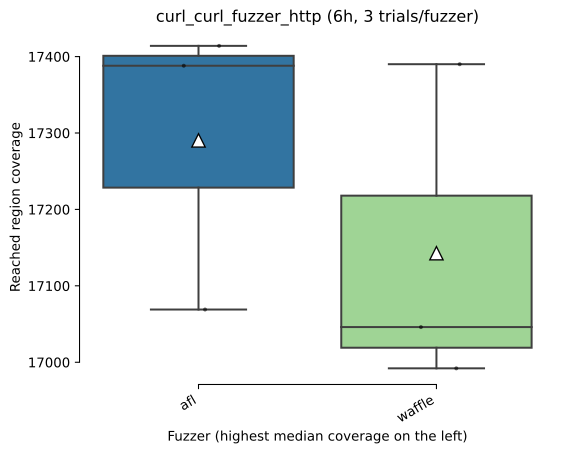
\includegraphics[width=\textwidth]{Chapter4/experimental/WA-cur/curl_curl_fuzzer_http_boxplot.png}
            \vspace*{-5mm}
            \caption{Waffle-AFL curl\_curl\_fuzzer\_http}
            \label{box:wac}
            \vspace*{5mm}
        \end{subfigure}
        ~
        \begin{subfigure}[t]{0.5\textwidth}
            \centering
            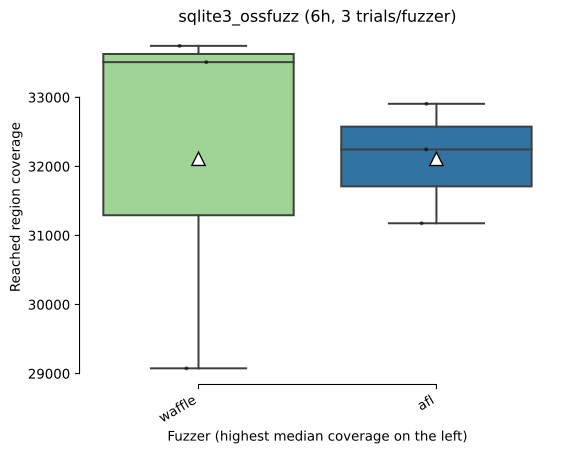
\includegraphics[width=\textwidth]{Chapter4/experimental/WA-sql/sqlite3_ossfuzz_boxplot.png}
            \vspace*{-5mm}
            \caption{Waffle-AFL sqlite3\_ossfuzz}
            \label{box:was}
            \vspace*{5mm}
        \end{subfigure}
    \end{adjustbox}
    \caption{Reached code coverage distribution (cont.)}
    % \label{fig:report-box}
\end{figure}

In the end, the number of unique findings of each fuzzer is shown in the last column. Overally speaking, Waffle outperforms AFL in fuzzing \textit{sqlite3}

% \begin{figure}[!t]
%     \begin{adjustbox}{center,max width=1.3\textwidth}
%         \begin{subfigure}[t]{0.55\textwidth}
%             \centering
%             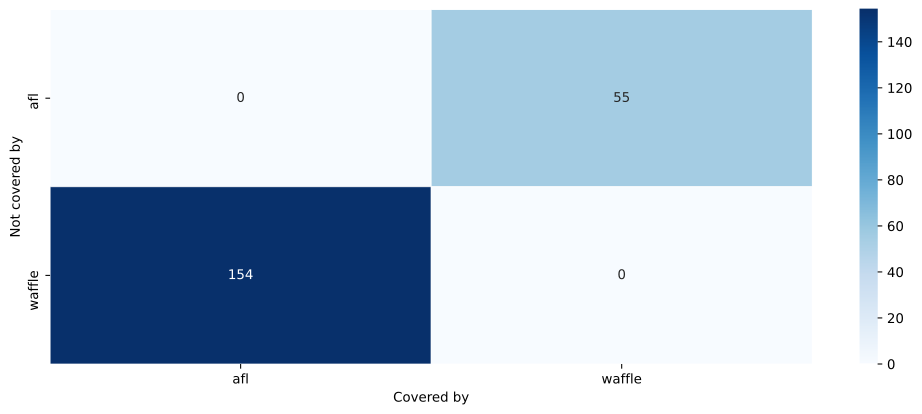
\includegraphics[width=\textwidth]{Chapter4/experimental/WA-cur/curl_curl_fuzzer_http_pairwise_unique_coverage_plot.png}
%             \vspace*{-5mm}
%             \caption{curl\_curl\_fuzzer\_http}
%             \label{unq:a}
%             \vspace*{5mm}
%         \end{subfigure}
%         ~
%         \begin{subfigure}[t]{0.55\textwidth}
%             \centering
%             \includegraphics[width=\textwidth]{Chapter4/experimental/WA-lib/libpng-1.2.56_pairwise_unique_coverage_plot.png}
%             \vspace*{-5mm}
%             \caption{libpng-1.2.56}
%             \label{unq:b}
%             \vspace*{5mm}
%         \end{subfigure}
%     \end{adjustbox}
%     ~
%     \begin{adjustbox}{center,max width=1.3\textwidth}
%         \begin{subfigure}[t]{0.55\textwidth}
%             \centering
%             \includegraphics[width=\textwidth]{Chapter4/experimental/WA-php/php_php-fuzz-execute_pairwise_unique_coverage_plot.png}
%             \vspace*{-5mm}
%             \caption{php\_php-fuzz-execute}
%             \label{unq:c}
%             \vspace*{5mm}
%         \end{subfigure}
%         ~
%         \begin{subfigure}[t]{0.55\textwidth}
%             \centering
%             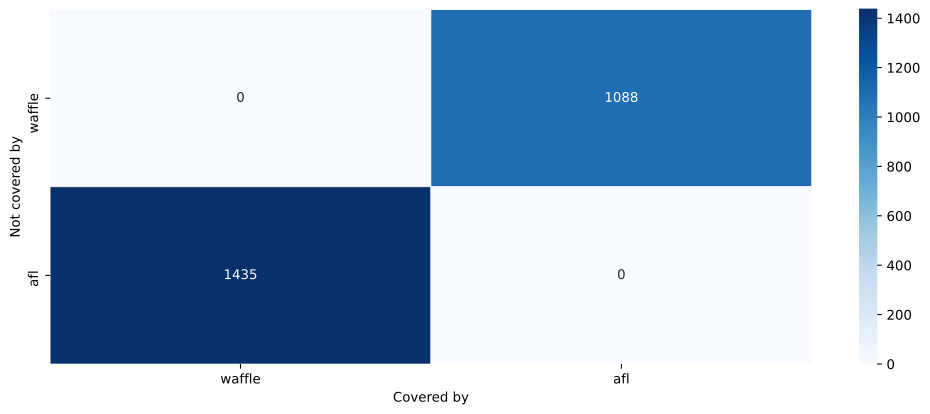
\includegraphics[width=\textwidth]{Chapter4/experimental/WA-sql/sqlite3_ossfuzz_pairwise_unique_coverage_plot.png}
%             \vspace*{-5mm}
%             \caption{sqlite3\_ossfuzz}
%             \label{unq:d}
%             \vspace*{5mm}
%         \end{subfigure}
%     \end{adjustbox}
%     ~
%     \begin{adjustbox}{center,max width=1.3\textwidth}
%         \begin{subfigure}[t]{0.55\textwidth}
%             \centering
%             \includegraphics[width=\textwidth]{Chapter4/experimental/WA-thr/openthread-2019-12-23_pairwise_unique_coverage_plot.png}
%             \vspace*{-5mm}
%             \caption{openthread-2019-12-23}
%             \label{unq:e}
%             \vspace*{5mm}
%         \end{subfigure}
%         ~
%         \begin{subfigure}[t]{0.55\textwidth}
%             \centering
%             \includegraphics[width=\textwidth]{Chapter4/experimental/WL-lib/libpng-1.2.56_pairwise_unique_coverage_plot.png}
%             \vspace*{-5mm}
%             \caption{libpng-1.2.56}
%             \label{unq:f}
%             \vspace*{5mm}
%         \end{subfigure}
%     \end{adjustbox}
%     ~
%     \begin{adjustbox}{center,max width=1.3\textwidth}
%         \begin{subfigure}[t]{0.55\textwidth}
%             \centering
%             \includegraphics[width=\textwidth]{Chapter4/experimental/WL-php/php_php-fuzz-execute_pairwise_unique_coverage_plot.png}
%             \vspace*{-5mm}
%             \caption{php\_php-fuzz-execute}
%             \label{unq:g}
%             \vspace*{5mm}
%         \end{subfigure}
%         ~
%         \begin{subfigure}[t]{0.55\textwidth}
%             \centering
%             \includegraphics[width=\textwidth]{Chapter4/experimental/WL-thr/openthread-2019-12-23_pairwise_unique_coverage_plot.png}
%             \vspace*{-5mm}
%             \caption{openthread-2019-12-23}
%             \label{unq:h}
%             \vspace*{5mm}
%         \end{subfigure}
%     \end{adjustbox}
%     \caption{The above figures displays the reached coverage in the end of the experiments. The green boxes represent Waffle's code coverage.}
%     \label{fig:report-unq}
% \end{figure}
